% The OVF E2E VIV Report

% Turning off "draft" mode on the report class turns off to do notes,
% chapter assignments, and completion percentages
\documentclass[draft]{report}

\usepackage{times}

\usepackage{ifpdf}
\usepackage{ifdraft}
\usepackage[utf8]{inputenc}
\usepackage{fnpct}
\usepackage{xcolor}
\usepackage[final]{graphicx} % always include images, even in draft mode
\usepackage{xspace}
\usepackage{colortbl}
\usepackage{longtable}
\usepackage{tabu}
\usepackage[inline]{enumitem}
\usepackage[final]{listings} % always include listings, even in draft mode

% Bibliography equipment for fancier citations of websites etc
\usepackage[%
  backend=bibtex      % biber or bibtex
%,style=authoryear    % Alphabeticalsch
 ,style=numeric-comp  % numerical-compressed
%,sorting=none        % no sorting
 ,sortcites=true      % some other example options ...
 ,block=none
 ,indexing=false
 ,citereset=none
 ,isbn=true
 ,url=true
 ,doi=true            % prints doi
 ,natbib=true         % if you need natbib functions
]{biblatex}
\addbibresource{bibliography.bib}

\setcounter{biburllcpenalty}{7000}
\setcounter{biburlucpenalty}{8000}

% BON listing style
\usepackage{color}
\usepackage{listings}


\newcommand{\comment}[1]{\textcolor{red}{#1}}
\definecolor{keywordcolor}{rgb}{0.5,0,0.33}
\definecolor{identifiercolor}{rgb}{0,0,0.75}
\definecolor{commentcolor}{rgb}{0.25,0.5,0.37}
\definecolor{commentcolor}{rgb}{0.3,0.3,0.3} 

\lstdefinelanguage{bon} {
  morekeywords={class_chart,indexing,explanation,part,query,command,constraint,
  end,deferred,effective,persistent,require,ensure,invariant,feature,class,
  static_diagram,component,old,not,inherit,delta,for_all,such_that,it_holds,Current,
  Lockset,when,monitors_for,max,concurrency,concurrent,guarded,locks,special,
  failure,sequential,atomic},
  morekeywords={[2]BOOLEAN,INTEGER,REAL,SEQUENCE}, 
  morekeywords={[3]},
  morecomment=[l]{--}, morestring=[b]", morestring=[d]'
  }[keywords,comments,strings]

\lstdefinestyle{bon}{language={bon},showstringspaces={false},
  basicstyle={\small\ttfamily\mdseries},
  keywordstyle={\color{keywordcolor}},
  keywordstyle={[2]\color{black}\bfseries},
  keywordstyle={[3]\color{black}\bfseries},
  identifierstyle={\color{identifiercolor}},
  commentstyle={\color{commentcolor}},
  frame=none}

\lstdefinestyle{bonbw}{language={bon},showstringspaces={false},
  basicstyle={\small\ttfamily\mdseries},
  keywordstyle={\color{black}},
  keywordstyle={[2]\color{black}\bfseries},
  keywordstyle={[3]\color{black}\bfseries},
  identifierstyle={\color{black}\mdseries},
  commentstyle={\color{black}},
  frame=none,
  columns=fullflexible,
  breaklines=true}
\lstset{style=bon, columns=fullflexible, keepspaces=true, frame=lines,
  captionpos=b, numbers=none} 

% custom colors
\colorlet{darkgreen}{green!35!black}
\colorlet{darkred}{red!45!black}

% shades of red and green that are distinguishable even with the most common
% kinds of color blindness
\colorlet{accessiblegreen}{green!55!black!70!blue!40!white}
\colorlet{accessiblered}{red!80!black!80!yellow!30!white}

\usepackage[margin=1in]{geometry}
\usepackage[defaultlines=4,all]{nowidow}
\usepackage[parfill]{parskip}

%% To Do Notes
\usepackage[obeyDraft, colorinlistoftodos, textwidth=\marginparwidth]{todonotes}

% individual colors for To Dos, feel free to change yours
\colorlet{tododmz}{green!50}
\colorlet{todokiniry}{red!50}
\colorlet{tododmwit}{orange!50}
\colorlet{todojkr}{blue!50}
\colorlet{todoprobinson}{purple!50}
\colorlet{todoacf}{cyan!50}
\colorlet{todogeneric}{yellow!50}

\newcounter{todocounter}
\newcommand{\todocount}[2][]{\stepcounter{todocounter}\todo[#1]{\thetodocounter:
    #2}}

% individual commands for To Dos
% usage: \todo<username>{Something to do.}
\newcommand{\tododmz}[1]{\todocount[color=tododmz]{#1}}
\newcommand{\todokiniry}[1]{\todocount[color=todokiniry]{#1}}
\newcommand{\tododmwit}[1]{\todocount[color=tododmwit]{#1}}
\newcommand{\todojkr}[1]{\todocount[color=todojkr]{#1}}
\newcommand{\todoprobinson}[1]{\todocount[color=todoprobinson]{#1}}
\newcommand{\todoacf}[1]{\todocount[color=todoacf]{#1}}
\newcommand{\todogeneric}[1]{\todocount[color=todogeneric]{#1}}

\ifpdf
\usepackage[draft=false,pdftex,colorlinks=true,urlcolor=blue,linkcolor=darkred,citecolor=darkgreen,bookmarks=false]{hyperref}
\else
\usepackage[dvips]{hyperref}
\fi


% define a macro \Autoref to allow multiple references to be passed to
% \autoref
\makeatletter
\newcommand\Autoref[1]{\@first@ref#1,@}
\def\@throw@dot#1.#2@{#1}% discard everything after the dot
\def\@set@refname#1{%    % set \@refname to autoefname+s using \getrefbykeydefault
    \edef\@tmp{\getrefbykeydefault{#1}{anchor}{}}%
    \def\@refname{\@nameuse{\expandafter\@throw@dot\@tmp.@autorefname}s}%
}
\def\@first@ref#1,#2{%
  \ifx#2@\autoref{#1}\let\@nextref\@gobble% only one ref, revert to normal \autoref
  \else%
    \@set@refname{#1}%  set \@refname to autoref name
    \@refname~\ref{#1}% add autoefname and first reference
    \let\@nextref\@next@ref% push processing to \@next@ref
  \fi%
  \@nextref#2%
}
\def\@next@ref#1,#2{%
   \ifx#2@ and~\ref{#1}\let\@nextref\@gobble% at end: print and+\ref and stop
   \else, \ref{#1}% print  ,+\ref and continue
   \fi%
   \@nextref#2%
}
\makeatother

\usepackage{lipsum}
\usepackage{soul}

% Modify the autoref names to be capitalized and not sub-sub-subby.
\renewcommand*{\chapterautorefname}{Chapter}
\renewcommand*{\sectionautorefname}{Section}
\renewcommand*{\subsectionautorefname}{Section}
\renewcommand*{\subsubsectionautorefname}{Section}

% Various definitions, from Aggelos E2E spec

\newcommand{\func}[1][\relax]{\ensuremath{\mathcal{F}_{\mathsf{#1}}}}
\newcommand{\fl}[1]{\mbox{\( \lfloor #1 \rfloor \)}}
\newcommand{\pair}[2]{\mbox{\(\langle #1,#2 \rangle\)}}

\newcommand{\mc}{\mathcal}
\newcommand{\Pro}{\mbox{\( \mathbf{ Prob } \)}}

\def\squareforqed{\hbox{\(\blacksquare\)}}
\def\qed{\ifmmode\squareforqed\else{\unskip\nobreak\hfill\penalty50\hskip1em\null\nobreak\hfil\squareforqed\parfillskip=0pt\finalhyphendemerits=0\endgraf}\fi}

\newtheorem{theorem}{Theorem}[section]
\newtheorem{assumption}{Complexity Assumption}
\newtheorem{lemma}[theorem]{Lemma}
\newtheorem{remark}{Remark}
\newtheorem{claim}{Claim}
\newtheorem{fact}[theorem]{Fact}
\newtheorem{definition}[theorem]{Definition}
\newtheorem{corollary}[theorem]{Corollary}
\newtheorem{proposition}[theorem]{Proposition}
\newenvironment{proof}{\noindent {\em Proof.}}{\medskip}

\def\PPT{{\rm PPT} }
\def\ff{\mathbb{F}}
\def\sbs{\subseteq}
\def\zz{\mathbb{Z}}
\def\E{\mathsf{E}}

%Functionalities
\newcommand{\fete}{\func[e2e]}%
\newcommand{\fbb}{\func[bb]}%
\newcommand{\fsauth}{\func[sauth]}%
\newcommand{\fauth}{\func[auth]}%
\newcommand{\fmail}{\func[mail]}%
\newcommand{\frnd}{\func[rnd]}%

%Parties
\def\EA{\mathsf{EA}}
\def\VT{\mathsf{V}}
\def\RB{\mathsf{RB}}
\def\VC{\mathsf{VC}}
\def\AU{\mathsf{AU}}

\def\Exec{\mathsf{Exec}}


%Commands
\def\Create{\mathtt{Create}}
\def\Sample{\mathtt{Sample}}
\def\FakeBallot{\mathtt{FakeBallot}}
\def\Deliver{\mathtt{Deliver}}
\def\Corrupt{\mathtt{Corrupt}}
\def\Verify{\mathtt{Verify}}
\def\Tally{\mathtt{Tally}}
\def\Vote{\mathtt{Vote}}
\def\RecordVote{\mathtt{RecordVote}}
\def\Append{\mathtt{Append}}
\def\Read{\mathtt{Read}}
\def\Send{\mathtt{Send}}
\def\Mail{\mathtt{Mail}}
\def\Audit{\mathtt{Audit}}
\def\VBB{\mathtt{VBB}}
\def\SendInit{\mathtt{SendInit}}
\def\GetRnd{\mathtt{GetRnd}}
\def\Select{\mathtt{Select}}
\def\RecordTally{\mathtt{RecordTally}}
\def\ReadTally{\mathtt{ReadTally}}
\def\Receipt{\mathtt{Receipt}}
\def\Result{\mathtt{Result}}
\def\ElectionFail{\mathtt{ElectionFail}}

% End of preamble

\title{The E2EVIV Report}
\author{Many People}

\begin{document}

% The title page has no visible page number, and the report resets page
% numbering on the next page so that the visible page numbers start from 1.
% One unfortunate side effect of this is that hyperref sees two different
% pages both named "1" and gets confused. See also
% http://tex.stackexchange.com/q/18924/16779
\hypersetup{pageanchor=false}
\maketitle
\hypersetup{pageanchor=true}

\tableofcontents

\clearpage
\ifdraft{\addcontentsline{toc}{chapter}{\ \ \ \ \hl{Note: Names following
    chapter titles are the currently-assigned writers; percentages
    following writer names are very rough estimates of the
    approximate percentage of completion. Some material factored 
    into the percentages may not yet appear in the generated report 
    because it needs to be brought in from external sources.} \\ \ \\
  List of To Do Items}
% temporarily here, so we have a centralized list of all the todo
% items in the document
\listoftodos[List of To Do Items]
}{}
\chapter{Executive Summary\ifdraft{ (Joe K./Susan) (0\%)}{}}
\label{chapter:executive_summary}

\begin{itemize}
\item framing of project \& methodology
\item who is involved
\item who funded it
\item goals and deliverables
\item feasibility
\item recommendation
\item ``why now'' coupled to history
\item why do existing systems suck
\item ``how'' what is E2E VIV (illustration)
\item five key mandatory properties: end-to-secure, verifiability,
  100\% accessible, high-assurance, transparent
\item crypto framing
\item architectural framing
\item RSE framing
\item conclusion and future phases
\end{itemize}
 % Joe K./Susan
\chapter{Introduction\ifdraft{ (Joe K./Susan) (70\%)}{}}
\label{chapter:introduction}

%=====================================================================
\section{The E2E VIV Project}

%~~~~~~~~~~~~~~~~~~~~~~~~~~~~~~~~~~~~~~~~~~~~~~~~~~~~~~~~~~~~~~~~~~~~~
\subsection{Situation}

In March 2013, Overseas Vote Foundation’s President and CEO began a
discussion with a small group of experienced, election integrity
technology advocates about how, if faced with having to specify an
Internet voting system, they would respond. Security concerns being
the primary reason for their general opposition to what they deemed
inadequate efforts of others to do so to date, it was nonetheless
agreed that taking on the question was crucial at the time. 

Gridlock is not unique to Washington politics, it is quite well known
around the topic of Internet Voting in the U.S. The scientific
community, federal agencies, cyber security specialists and certain
organized activists have strongly advised against exposing the ballots
of the most powerful nation on earth to the seemingly endless range of
cyber threats, which run rampant on today’s Internet. 

Nevertheless, faced with ongoing challenges to serve their
constituencies in modern and efficient ways, and having experienced
the everyday efficiencies of technology throughout their lives, when
seeking new and improved election systems, election officials often
want to consider Internet-based technologies. In the current climate
of economic austerity, innovation in elections is rare. Our election
officials are trapped in a technology no-man’s land of ongoing support
payments for outdated voting systems, compounded by no means of
certifying new voting systems they would like.

Election integrity advocates cite that secure, tested, certified
remote voting systems that election officials envision aren’t
available. The scientific community does not consider online ballot
return systems secure, nor are they certified. As a result, email has
become the default stopgap method for moving ballots online, although
it does not provide any of the benefits that a secure, full-featured
voting system would provide. Email is demonstrably weak on security,
yet election officials and voters are using it regularly to transmit
ballots because viable alternatives are not available. Examination of
new and better ways to use technology to meet specific voting needs,
for example, that of the remote overseas citizen, military and
disabled is needed. 

Existing vendors of Internet voting technologies, whose systems are
neither tested nor certified, would like to openly market and sell
their systems within the U.S. and not face the resistance of the
election integrity advocates. No agreement on how to proceed, a
years-long history of mediocre attempts, ongoing animosity between
stakeholder parties, and a general lack of research on the current
questions could well-describe the situation.

%~~~~~~~~~~~~~~~~~~~~~~~~~~~~~~~~~~~~~~~~~~~~~~~~~~~~~~~~~~~~~~~~~~~~~
\subsection{A Proposed Solution}

Within this climate, a project proposal was written and funding
provided by The Democracy Fund, a Washington D.C. based philanthropic
organization whose stated objective is to “...invest in organizations
working to ensure that our political system is responsive to the
priorities of the American public and has the capacity to meet the
greatest challenges facing our country.” 

A project intent on examining the future of voting and how it might be
executed securely online fit neatly into the strategic purview of the
fund; one that approached the question of Internet-voting from a
research perspective, that sought to fill in the gaps of the many open
questions plaguing the discussion was regarded by the supporting
organization as a positive endeavor. 

According to Joe Goldman, Director of the Democracy Fund, “The
significance of this project will be in its ability to break open the
conversation from its current stalemate and include all sides in a
constructive project to openly examine and research what is really
needed by voters and election officials, and to determine whether this
form of voting can meet those needs and still guarantee security of
the election. Equally important, it will identify potential tradeoffs
and shortcomings that represent the diverse range of values we hold
dear in our elections.”

On December 19, 2013, Overseas Vote Foundation\footnote{Since the
  start of the study, Overseas Vote Foundation has been renamed as
  “Overseas Vote”, an initiative of U.S. Vote Foundation.} (OVF), a
nonpartisan, nonprofit organization dedicated to overseas and military
voter participation announced the launch of the project, which was
called the End-to-End Verifiable Internet Voting: Specification and
Feasibility Assessment Study (E2E VIV Project). Its stated aim was to
examine a form of remote voting that enables a so-called “end-to-end
verifiability” (E2E) property. A unique team of experts in computer
science, usability, and auditing together with a selection of local
election officials from key counties around the U.S. assembled for the
study.

They agreed to focus their efforts to produce a system specification
and set of testing scenarios, which if they meet the requirements for
security, auditability, and usability, would then be placed in the
public domain. At the same time, their intent was to demonstrate that
confidence in a voting system is built on a willingness to verify its
security through testing and transparency. 

There is an historical misunderstanding in the U.S. election community
that the E2E VIV Project aimed to correct: that our country’s best
scientists are not against technology advancements, nor are they
inherently at odds with the election officials who seek technology
improvements to meet their administrative challenges. Rather, that the
U.S. scientific community takes issue with unproven claims of security
regarding existing systems that are not publicly tested or vetted. The
study aimed to recalibrate this situation. 

The group of scientific leaders on the project has often pointed out
security vulnerabilities in past systems, however, in the face of the
E2E VIV Project, they agreed on one thing: that if Internet Voting
(IV) does happen, it should be in a system that takes advantage of
end-to-end verifiability and auditability.

%~~~~~~~~~~~~~~~~~~~~~~~~~~~~~~~~~~~~~~~~~~~~~~~~~~~~~~~~~~~~~~~~~~~~~
\subsection{Definition}

The term E2E is often used casually without
precision. E2E-verifiability is considered a property of an election
and for the purposes of the study, an E2E-verifiable election has two
important components: first, that voters can individually check that
their ballots are cast as they intend; and second, that anyone can
check that all of the cast ballots have been accurately
tallied\footnote{Definition from Dr.~Josh Benaloh, Senior
  Cryptographer at Microsoft Research.}.

While systems of this nature have been developed in the past, none
have been broadly used or successfully commercialized; the E2E VIV
Project would make a concerted effort to be informed by these past
efforts and build upon them as appropriate. Usability factors were
also considered from the outset of the study to address the
significant challenges faced by remote and disabled voters when using
such systems to participate. A viable outcome of this study with
respect to security, auditability, and usability is intended to enable
development efforts to ensue.

For those concerned with election integrity, there is a justifiably
negative reflex in response to IV: it takes all of the problems with
current remote voting systems and adds all of the problems and
security vulnerabilities of the Internet.  

The E2E VIV Project sought to potentially make the case that use of
the Internet enables and facilitates the introduction of
E2E-verifiability (E2EV) and that the benefits of E2EV may be able to
overcome the vulnerabilities introduced by using the Internet. No
participant on this project discounted the concerns of voting over the
Internet, nor did or do they view E2EV as a magic sauce that makes the
Internet secure. Nevertheless they believe that E2EV warrants
examination in regards to the properties it achieves. These properties
are achieved even when votes are cast on untrusted devices like PCs
and transmitted over an untrusted medium such as the Internet.

The E2E VIV Project does not attempt to make the Internet
secure. Instead, E2EV negates many (although not all) of the risks of
voting via the Internet while introducing substantial new benefits
that are not found in currently deployed voting systems.

%=====================================================================
\section{Goals and Objectives}

%~~~~~~~~~~~~~~~~~~~~~~~~~~~~~~~~~~~~~~~~~~~~~~~~~~~~~~~~~~~~~~~~~~~~~
\subsection{Shared Goals}

Election officials and scientists involved in elections \textbf{share}
the overall goals: that voting systems can be proven secure,
auditable, verifiable, and accessible.

This project is evidence that the needs and requests of election
officials to explore optimum ways of serving remote voters are of deep
concern to the scientific community, that they have a great motivation
to address these questions when given a constructive opportunity to do
so, and that they would like to work together, not at opposite ends,
to examine the possibilities in this realm.

%~~~~~~~~~~~~~~~~~~~~~~~~~~~~~~~~~~~~~~~~~~~~~~~~~~~~~~~~~~~~~~~~~~~~~ 
\subsection{Project Goal}

Our goal is to specify and define a system and its testing scenarios
for an online voting method that can provide both security and
confidence to voters that their selections are accurately recorded and
counted. Our assertion is that E2E-verifiability negates many,
although not all, of the risks of voting via the Internet while
introducing substantial new benefits that are not found in currently
deployed voting systems.

The project team presumes that if E2E VIV is a possible answer, or a
step toward one, we will find out and we will see if it can answer the
needs of many voters and election officials. If not, we will still
gain specific knowledge about the shortcomings, which can be further
acted upon in the future. 

%~~~~~~~~~~~~~~~~~~~~~~~~~~~~~~~~~~~~~~~~~~~~~~~~~~~~~~~~~~~~~~~~~~~~~
\subsection{Additional Objectives}

Presentation and discussion of the report with key stakeholders,
integrating their feedback, and garnering their cceptance of the
report (see below in Success section) are additional core objectives
of the project. 

%~~~~~~~~~~~~~~~~~~~~~~~~~~~~~~~~~~~~~~~~~~~~~~~~~~~~~~~~~~~~~~~~~~~~~
\subsection{Deliverables}

The main deliverable of the E2E VIV Project is the development of a
``whole product solution'' specification (or simply specification for
short) for a trustworthy E2E VIV election system.

We have produced a report presenting a system specification to create
a secure E2E VIV system, a set of testing specifications to
demonstrate the security, a set of guidelines for system usability,
accessibility, and testing. Additional topics and analyses may be
considered and discussed in the report, such as legal and
administrative challenges, and ballot secrecy, privacy, and
confidentiality.

%~~~~~~~~~~~~~~~~~~~~~~~~~~~~~~~~~~~~~~~~~~~~~~~~~~~~~~~~~~~~~~~~~~~~~
\subsection{A First Step}

This project represents step one in an examination of whether one day
this might be possible. Our current plan is to examine the potential
for an E2E VIV remote voting system together with election officials,
taking into close account their needs and the needs of disabled
voters. If a system can one day be developed based on these
principles, then we want to know. We need the answers that this
project will bring before we can say whether we, or anyone, will build
any new system. A viable outcome of this study with respect to
security, auditability, and usability will enable development efforts
to ensue.

%~~~~~~~~~~~~~~~~~~~~~~~~~~~~~~~~~~~~~~~~~~~~~~~~~~~~~~~~~~~~~~~~~~~~~
\subsection{Success}

Beyond judging the outcome – the fact that this project takes a
research and testing-based approach to a problem that has been “in
stalemate mode” will result, we believe, in stimulating election
development overall. The election industry is operating in a
traditional paradigm with only a few vendors able to survive, albeit
demand to move away from outdated, expensive, hardware-oriented
solutions.

It would be considered a success to specify a system and testing for a
usable, secure E2E verifiable remote voting technology, to identify
its strengths and weaknesses and reasons to pursue or not pursue this
approach to remote and/or disabled citizen voting.

However, from the beginning is was clear that if the project
determines that the technology is weak and should not be developed, it
would be a different outcome, but also one with many useful
implications. 

Success of the project can only be determined if the specification is
one that is: 1)~supported by the vast majority the expert teams,
including the technical, usability, testing, and research teams;
2)~endorsed by the vast majority of the advisory council, and;
3)~endorsed by the major stakeholders in elections administration as
represented by the project's local election officials.

Additionally, the E2E VIV Project expects to receive support and
endorsement from many members of the electronic voting activism
community, as represented by key members of the Election Verification
Network and the Verified Voting Foundation.

The specification will be of a form with sufficient detail such that
the following requirements are fulfilled:
\begin{description}
\item[Independent Implementation] The specification must be of
  sufficient detail and clarity that an implementation of the election
  system must be possible by an independent party without extensive
  dialog with participants in the project.
\item[Independent Validation] It must be possible for a moderately
  proficient IT expert to objectively determine, in a reasonable time
  frame with reasonable cost, if any election system constructed which
  claims to fulfill the specification.
\item[Evidence-Based Decisions] Every decision made in the crafting of
  the specification must be objectively justifiable and the evidence
  for the decision must be traceable. 
\end{description}

%~~~~~~~~~~~~~~~~~~~~~~~~~~~~~~~~~~~~~~~~~~~~~~~~~~~~~~~~~~~~~~~~~~~~~
\subsection{Scope}

The original project was tightly limited to involve system
specification and testing only. No system development was envisioned
in this phase beyond mockups to help test usability. However, this
changed early on in the project when Joe Kiniry of Galois, Inc. came
on board to manage the project and its team. 

The Galois engineers brought significant expertise to the project and
set about to develop a set of rigorous engineering artifacts
``demonstrators'' fit for refinement into a working election system, and
against which third parties can perform independent validation and
verification. According to Galois, demonstrators are technical
artifacts from the point of view of definition and constructions, but
non-technical artifacts from the point of view of
demonstration. Galois suggests that all demonstrators developed using
Galois IR\&D funding be: 
\begin{itemize}
\item developed in a completely transparent and public fashion within
  the Galois GitHub Organization, 
\item cross-referenced, and thus traceable to and from, all
  specification aspects (from domain models to behavioral design
  specifications), are replicated into the E2E VIV GitHub
  Organization, and
\item are licensed under either a mainstream Open Source license with
  a strong community or an alternative license tuned to the elections
  community.
\end{itemize}

Significantly, Galois is a leader in the process of computing on data
while it remains encrypted, and in the automated generation,
validation and synthesis of high assurance cryptographic
solutions. They excel in multiple areas of cryptographic
implementation, all of which can be applied to the challenge of
developing secure and usable E2E VIV voting.

Relevance of Galois’ work to the project was explicit: the aim to
apply cutting edge computer science and mathematics to solve difficult
technological problems was a clear definition of what was needed to
solve the secure, verifiable election systems development
challenge. Galois’ management agreed to donate a significant portion
of engineering time to the project in order to build “demonstrators”
that would be used to prove the concepts of E2EV and to further
examine security and usability.

%=====================================================================
\section{People}

Inherent in the E2E VIV Project was the opportunity to combine the
abilities, knowledge, experience and expertise of a diverse group of
technologists, computer scientists and election officials involved in
election integrity together to form the overall project
team. Technical, usability, testing and local election official
sub-teams were formed for ease of communication. The technical team
has decades of experience in E2E technology, cryptography, usability,
and testing. An Advisory Council was established to broaden the
communication with interested members of the election community. 

Overseas Vote Foundation (OVF), as the official grantee, was
responsible the overall project conception, proposal development,
presentations, communications, management, team recruitment,
contractual obligations, public relations, events and budgeting. Deep
experience in the arena of overseas and military voting, absentee
voting, community building, voter survey research, election reform and
communications gave OVF a unique edge in managing the project. 

Galois, Inc. provided the technical and engineering project
management. Named as the technical project manager, Joe Kiniry,
working as a Principal Investigator at Galois facilitated the
communication and decision-making of the expert teams. He became the
main author and editor of the report and ran all engineering projects
and usability aspects of the study. 

%~~~~~~~~~~~~~~~~~~~~~~~~~~~~~~~~~~~~~~~~~~~~~~~~~~~~~~~~~~~~~~~~~~~~~
\subsection{Team Members}

\textbf{Project Manager:} Susan Dzieduszycka-Suinat, Overseas Vote Foundation

\textbf{Lead Technical Project Manager:} Dr. Joseph Kiniry, Galois

\textbf{Technical Team}

Dr. Josh Benaloh
Senior Cryptographer, Microsoft Research
 
Dr. David R. Jefferson
Lawrence Livermore National Laboratory
 
Dr. Doug W. Jones
Associate Professor, Department of Computer Science, University of Iowa
 
Dr. Aggelos Kiayias
Associate Professor, Computer Science and Engineering, University of Connecticut
 
Dr. Olivier Pereira
Professor, Institute of Information and Communication Technologies, Electronics and Applied Mathematics, Ecole Polytechnique de Louvain
 
Dr. Poorvi Vora
Associate Professor, Department of Computer Science, The George Washington University
 
Dr. David Wagner
Professor, EECS Computer Science Division, University of California Berkeley
 
Dr. Dan Wallach
Professor, Department of Computer Science, Rice University
 
\textbf{Usability Team}

Keith Instone
User Experience Consultant

Morgan Miller [ KEEP? ]
Usability Analyst, Experience Lab

Dr. Judith Murray
Research Consultant
 
\textbf{Election Auditing}

Dr. Philip Stark
Professor and Chair of Statistics, University of California Berkeley
 
\textbf{Testing Team}

Dr. Duncan Buell
Professor of Computer Science and Engineering, University of South Carolina
 
Andrew Regenscheid
Mathematician, National Institute of Standards and Technology
 
\textbf{Advisory Council}

Dr. Ben Adida
 
Dr. Michael Clarkson
Assistant Professor of Computer Science, The George Washington University
 
Dr. J. Alex Halderman
Assistant Professor of Computer Science and Engineering, University of Michigan
 
Candice Hoke
Professor of Law, Cleveland State University
 
Dr. Ron Rivest
Vannevar Bush Professor of Computer Science, Massachusetts Institute of Technology
 
Noel Runyan
Primary Consultant, Personal Data Systems
 
Dr. Peter Ryan
Professor in Applied Security, University of Luxembourg
 
Dr. Barbara Simons
Research Staff Member, IBM Research (retired)
 
Dr. Vanessa Teague
Research Fellow, Department of Computing and Information Systems, University of Melbourne
 
John Wack
Voting Systems Standards, National Institute of Standards and Technology
 
Dr. Filip Zagorski
Assistant Professor of Computer Science, Wroclaw University of Technology
 
\textbf{Local Election Officials}

Lori Augina
Director of Elections, Washington State, Secretary of State

Rachel Bohman
Former Hennepin County Elections Manager (Minnesota)

Judd Choate
Director of Elections, Colorado, Secretary of State

Dana Debeauvoir
Travis County Clerk (Texas)
 
Mark Earley
Voting Systems Manager, Leon County (Florida)
 
Dean Logan
Los Angeles Registrar-Recorder/County Clerk (California)

Stuart Holmes
Election Information Systems Supervisor, Office of the Secretary of State (Washington)
 
Dr. Lois H. Neuman
Chair, Board of Supervisors of Elections, City of Rockville (Maryland)
 
Roman Montoya
Deputy County Clerk, Bernalillo County (New Mexico)
 
Tammy Patrick
Senior Advisor to the Democracy Project, Bipartisan Policy Center and Former Federal Compliance Officer Maricopa County (Arizona)
 
\textbf{Overseas Vote Foundation Support Team}

Susan Dzieduszycka-Suinat
President and CEO
 
Paul McGuire
Legal Counsel and Secretary of the Board
 
Richard Vogt
Treasurer and Chief Financial Officer

Capstone Project Team, Carnegie Mellon University, Heinz College,
School of Information Systems \& Management; Master of Information
Systems Management and Master of Science in Information Security
Policy and Management: in early 2014, a Capstone Team was assigned to
the project team to assist on the Comparative Analysis of E2E systems.

\textbf{Unofficial Project Members/Stakeholder Groups}

Although not on the official project team, it was widely acknowledged
that there were several communities relevant to the E2E VIV Project
outside of those represented on the expert teams and that interaction
with members of these communities was essential. These included: 

\begin{itemize}
\item Advocates
\item Standards Bodies
\item Vendors
\item Hackers and Hacktivists
\item Election Officials 
\item Citizens
\end{itemize}

\todokiniry{Joe: Do you want to say anything about these groups?
  Should we remove this last paragraph and this list? -Susan}

%=====================================================================
\section{Methodology}

\todokiniry{Galois to write this section.}

%=====================================================================
\section{Outcome}

The E2E VIV Project produced a System Specification Development and
Documentation (referred to as a technical report for short) including
a Whole Product Solution Specification for an E2E VIV Election System
(referred to as a election system for short). The assessment of the
system by the expert team has had two possible outcomes. 

\begin{enumerate}
\item Positively, the majority of the expert team may decide that the
  specified election system meets all of the requirements set forth by
  the charter of the group. This outcome would indicate that OVF might
  potentially move forward to ensure that the election system is
  developed and, potentially, deployed.
\item Negatively, the majority of the expert team may decide that the
  specified election system does not meet all of the requirements set
  forth by the charter of the group. This outcome indicates that
  further funding to design or construct such an election system is,
  for the moment, unwise and that the community believes that
  designing a usable and secure election system is still an open
  scientific, not engineering, challenge. 
\end{enumerate}

Fulfilling the usability and security requirements would not be
sufficient for a positive assessment by the expert team. A full system
specification that is usable and secure may be, for example, far to
expensive to build, too difficult to deploy and manage, or mandate too
much expertise from election officials to operate. Social
non-functional requirements may trump technical functional
requirements. 

The Whole Product Solution Specification is written in one or more
specification languages that cover the technical needs of the E2E VIV
Project, particularly with regards to third party high-assurance
verification and validation of implementations. Galois recommended
using Alloy [10], RAISE [9], or PVS [18] to codify a formal domain
model, BON [21] to specify the election system's informal domain
model, requirements, architecture, and design, and F [8] and Cryptol
[4] to specify election system protocols. 

%~~~~~~~~~~~~~~~~~~~~~~~~~~~~~~~~~~~~~~~~~~~~~~~~~~~~~~~~~~~~~~~~~~~~~
\subsection{Deliverables}

A set of reports and a set of demonstrators were produced. Some
elements and report section where non-technical and others not. 

Galois contends that all project results should be SMART: 
\begin{itemize}
\item Specific: the determination of whether a result is accomplished
  is as objective as possible; 
\item Measurable: major results have a tracking dashboard on the
  project website and are updated and reviewed weekly; 
\item Attainable: E2E VIV Project participants believe they can
  achieve the results they propose; 
\item Relevant: results contribute to the priorities, goals, or
  on-going; operation of the project, and offer clear value to the
  project; and 
\item Trackable: progress toward the achievement of a result is
  monitored, including project budget. 
\end{itemize}

Moreover, each result must have a customer. A customer is an
individual or group who will negotiate a result and who will be
actively engaged. They will truly care that the result is achieved and
work to make us all successful in doing so. The customers of the E2E
VIV Project are the Local and State Election Officials. 

%~~~~~~~~~~~~~~~~~~~~~~~~~~~~~~~~~~~~~~~~~~~~~~~~~~~~~~~~~~~~~~~~~~~~~
\subsection{User Interface Design}

The user interface (or UI for short) of the E2E VIV election system is
the critical factor in ensuring that the system is both usable and
secure. Consequently, a detailed UI design informed by usability
testing, is a mandatory component of the system specification.

\todokiniry{Joe: Are you putting forward a “detailed UI design” –
  please adjust this as needed... and finish this section. I cannot
  finish on Outcomes.... -Susan}

%=====================================================================
\section{Next Steps}

\todokiniry{Joe: I don’t know what exactly you envisioned in “next
  steps” in this Introduction, but I am not sure about having it
  covered in this section. I would recommend it at the conclusion of
  the report and as part of the Executive Summary. -Susan}
 % Joe K./Susan
\chapter{Remote Voting\ifdraft{ (Philip) (30\%)}{}}
\label{chapter:remote_voting}

\section{Rationale}
\subsection{Geographic Dispersion}
\subsection{Accessibility}
\subsection{UOCAVA}
\subsection{Early Voting}
\subsection{Expectations}
\section{History}
\section{Current Practice}
\subsection{Integration with Local Elections}
\section{Shortcomings of Current Practice}
\subsection{Use of Communication/Internet}
\subsection{Accessibility and Usability}
\subsection{Auditing}
\subsubsection{Current Practice}
\subsubsection{Digital vs. Physical}
\subsubsection{Risk-Limiting Audits}
 % Philip
\chapter{E2E VIV Explained\ifdraft{ (Philip/Daniel/Adam) (25\%)}{}}
\label{chapter:e2e_viv_explained}

As discussed in \autoref{chapter:remote_voting}, there are several
difficulties with current voting processes: voters with disabilities cannot
vote unassisted, communication channels with remote voters are slow and
unreliable, vote tallying is labor-intensive and error-prone, and
election audits are costly. Additionally, there is little visibility into
the election process, meaning that individual voters and, in some cases,
even auditors, must trust the reports of election officials and voting
hardware vendors on election outcomes and processes. Election officials are
naturally seeking technology that can mitigate these problems, such as
automated, computer-based vote tallying to reduce tallying and auditing
costs, computerized ballot completion with accessibility technology to
assist disabled voters, Internet-based vote submission to increase the speed
and reliability of communicating with remote voters, and cryptographic
techniques for providing visibility without violating voter privacy. Below,
we give an overview of the goals of these technologies, discuss their
success at these goals, and highlight some common pitfalls.

\section{IV, VIV, E2E}

The core idea of Internet voting is deceptively simple: take a system that
allows remote voting via postal mail---which is already done in many
places---and replace some or all uses of postal mail in that process with
Internet-based delivery mechanisms. The draw of this idea is clear: messages
can be sent between election officials and voters in seconds, no matter how
distant, instead of weeks, and messages in typical Internet communication
methods are rarely lost, while up to half of overseas postal messages get
lost.

The general process is something like this:

\newcommand\stepref[1]{\hyperref[#1]{step~\ref*{#1}}}
\begin{enumerate}
  \item\label{enum:setup} Well before the election, officials compile a list
    of registered voters. They use this to populate a central database with
    contact information, details about what each voter's ballot should
    contain, and so forth. General instructions and other information about
    the election may be broadcast at or near this time---for example, via a
    central website.
  \item\label{enum:share secrets} Election officials contact each voter
    individually to set up some shared, but secret, information specific to
    that voter. For example, this might include an empty ballot with secret
    numbers associated with each candidate; or a cryptographic key-pair that
    the voter can use during communications with the officials. This is
    sometimes done by traditional means (like postal mail) and sometimes not
    done at all.
  \item\label{enum:send blank ballot} Once a means of communication is
    established in \stepref{enum:share secrets}, the election officials send
    the voter a blank ballot.
  \item\label{enum:complete ballot} The voter fills out the blank ballot on
    their computer, perhaps using custom software.
  \item\label{enum:send completed ballot} Again using the communication
    method established in \stepref{enum:share secrets}, the voter sends the
    completed ballot back to the election officials. Many systems have an
    additional step in which the election officials confirm receipt of the
    ballot.
  \item\label{enum:tally} After the election is over, all ballots sent in
    are tallied, and the outcome of the election is announced. In some
    systems, other supplemental information is often announced, such as
    whose votes were counted.
\end{enumerate}

Unfortunately, simply switching to Internet-based communication does not
solve all the problems discussed above, and introduces new problems of its
own.

\tododmwit{expand each of these}
\begin{description}
  \item[Secure transport] For the integrity of the vote, it is important
    that the empty ballot sent in \stepref{enum:send blank ballot} and the
    completed ballot sent in \stepref{enum:send completed ballot} arrive at
    their destination unmodified. The Internet includes a lot of hardware
    that is controlled by neither the election officials nor the voter, so
    ensuring this property can be quite a challenge. Some systems use a
    different communication channel in \stepref{enum:share secrets} to give
    greater confidence in this property, using information communicated by
    mail to cross-check information communicated over the Internet.
  \item[Private transport] Normally, votes are anonymous---there is no
    connection between a cast vote and the person who cast it. However,
    extant Internet communication protocols cannot support this privacy
    guarantee (and vote-by-mail systems typically sacrifice this property as
    well).
  \item[Attack surfaces] The voter is presumably using his own computer.
    It is possible that his computer has been taken over by somebody else.
    This kind of problem is completely fresh compared to paper voting.
  \item[Verifiability] Voters should be able to independently verify that
    their votes were cast and counted correctly, without needing to place
    trust in the communication medium or the election officials. Auditors
    should be able to check that the election was executed correctly without
    trusting the voting hardware and software vendors. Paper ballots support
    auditing well, but make individual voter confidence difficult.
\end{description}

\section{E2E Election Rituals}
\subsection{Pre-Election Phase}
\subsection{Voting}
\subsection{Post-Election Phase}
\section{Shortcomings and Expectations of E2EVIV}
\subsection{Access to Communication/Internet}
\subsection{Accessibility}
\subsection{Usability}
\section{E2E VIV in Practice}
\tododmwit{This section should be filled in with material from
  history.tex and comparative\_analysis.tex, and then history.tex and
  comparative\_analysis.tex should be ``retired'' and their resources
  moved into e2e\_viv\_explained\_resources.}
\section{Limitations of Existing Systems}
 % Philip/Daniel
\chapter{Required Properties of E2E Systems\ifdraft{ (Dan) (100\%)}{}}
\label{chapter:required_properties}

In August 2010, the U.S. Election Assistance Commission issued a set
of testing requirements for UOCAVA remote electronic voting system
pilot projects~\cite{eac-uocava2010}. The general categories of
requirements specified by the EAC included functional requirements,
such as the need for the system to produce paper records of voter
choices and generate human-readable ballot images; requirements on
software development, such as allowable programming languages and
coding conventions; usability, accessibility and privacy requirements,
such as that a voter's ballot choices must remain private and that
provisions must be made to support voters with disabilities; security
requirements, including logging requirements, requirements on
communications security within the system, and requirements on
physical security and penetration resistance; quality assurance
requirements describing the testing that must be done on the systems;
and requirements about configuration management mechanisms, technical
information, and documentation to be provided by system vendors.

The EAC requirements have some serious shortcomings, one of which is
that several of the requirements seem arbitrary. For example, they
specify (in Section 2.1 of the requirements document) that the voting
system shall achieve a target error rate of no more than one in
10,000,000 ballot positions, with a maximum acceptable error rate in
the test process of one in 500,000 ballot positions, without any
justification for those numbers. They further specify (in Sections
2.1.1.1--2) that ``memory hardware, such as semiconductor devices and
magnetic storage media, shall be accurate'' and that ``the design of
equipment in all voting systems shall provide for protection against
mechanical, thermal, and electromagnetic stresses that impact voting
system accuracy'' without any guidance on how to evaluate such
accuracy or protective ability.

In addition to these shortcomings, some of the EAC requirements are
inappropriate or invalid. The most obvious example of this is the set
of requirements that mandate specific ``structured programming''
characteristics of software implementation languages (Sections 4.1 and
4.4), which seem to eliminate functional programming languages such as
Haskell and Erlang---widely used in implementing high-assurance
systems---from consideration entirely.

If these issues were addressed, the EAC requirements could serve as a
solid baseline set of requirements for remote electronic voting
systems; effectively, addressing the ``IV'' in ``E2E-VIV''. However,
they are not strong enough to guarantee end-to-end verifiability,
which---as previously discussed---is essential when considering
Internet voting systems for use in real elections.  Thus, we describe
here a set of required properties for E2E-VIV systems that has
significant overlap with the EAC requirements.

The set of E2E-VIV requirements can be broadly divided into two
groups: \emph{technical requirements} and \emph{non-functional
  requirements}. Technical requirements are those that can be directly
addressed by the design and implementation of the system, such as
authentication requirements for voters and election
officials. Non-functional requirements are those that are imposed on
the system by external entities or where the system depends on
external behaviors outside its control, such as specific election
certification guidelines and operational procedures. Each of these
groups is itself divided into several categories, and
\autoref{fig:e2eviv_requirements_hierarchy} gives a high-level
overview of these.

\begin{figure}
\begin{center}
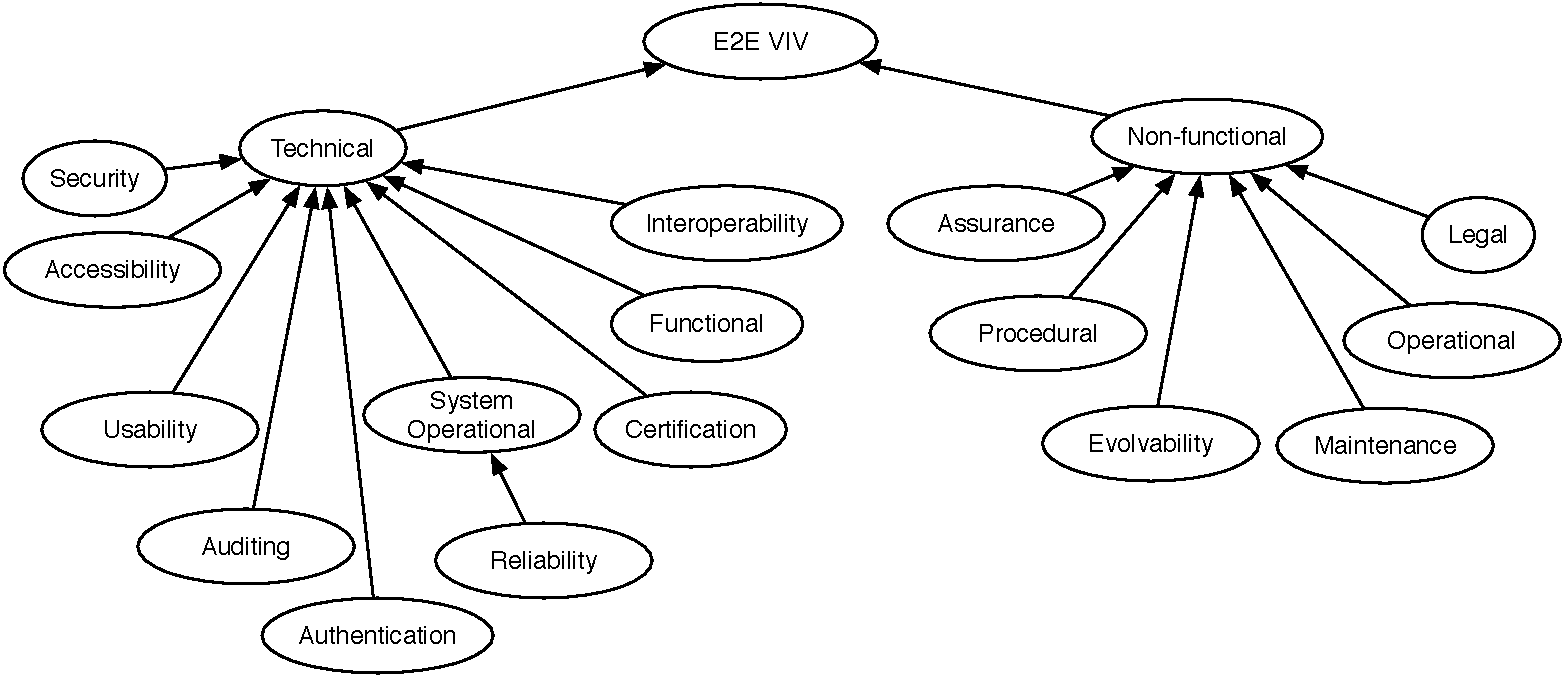
\includegraphics[width=6in]{required_properties_resources/hierarchy}
\end{center}
\caption{The hierarchy of requirements for E2E-VIV systems.}
\label{fig:e2eviv_requirements_hierarchy}
\end{figure}

The following is a high-level description of the categories and many
of the requirements within each; \autoref{appendix:bon_requirements}
contains a complete listing of all E2E-VIV system requirements
expressed in the Business Object Notation.

\section{Technical Requirements}
There are ten categories of technical requirements for E2E-VIV
systems: functional, accessibility, usability, security,
authentication, auditing, system operational, reliability,
interoperability, and certification. 

\subsection{Functional} 
\label{sec:functional}

The functional requirements of an E2E-VIV system deal primarily with
the casting and recording of ballots and associated voter records. One
important requirement is that there must be a correspondence between
the recorded ballots and the voters that are listed as having voted; a
ballot cannot be recorded without a voter casting it, and a voter
cannot be listed as having voted without casting a ballot. Similarly,
if a voter is informed by the system that her ballot has been
successfully cast, the system must correctly retain the record of her
having voted and her cast ballot information even in the event of
server failures.

Another functional requirement is the property of \emph{receipt
  freedom}: it must be impossible for a voter to prove to anybody any
information regarding how she voted her ballot, beyond what can be
mathematically deduced from the final distribution of votes. For
example, if a referendum passes with 100\% of the vote, there is no
way to hide the fact that every voter approved of the referendum;
however, if the result is mixed, it must be impossible for any
individual voter to prove how she voted.  This must be the case even
when the voter can create digital evidence of her actions by, for
example, video recording the ballot casting process or photographing a
completed ballot.

Note that there is no such E2E protocol in the literature. In order
for this requirement to be fulfilled, any protocol must allow the
voter to vote multiple times.  Yet, it must also allow it to appear
that the video-recorded vote was cast, hence its encryption must be
among those counted in a verifiable manner. Yet, this vote must not
count, and the later vote should replace it. This represents a
significant research challenge for cryptographic protocol designers.

In some elections voters are allowed to cast multiple ballots with
only the last cast ballot counting toward the final election tally,
while in others voters are prohibited from casting multiple
ballots. The system must accommodate both of these election formats,
ensuring that only the last cast ballot is counted for each voter when
multiple ballots are allowed and ensuring that each voter casts at
most one ballot otherwise.

Maintaining voter anonymity is critical, so it must be impossible
after the election to reconstruct a link between a cast ballot and any
identifying information about the voter who cast it. However, in
systems that support the casting of multiple ballots, it is important
to maintain links between voters and their ballots \emph{during} the
election to ensure that later ballots replace the correct earlier
ballots. To balance these concerns, any link between a ballot and the
voter who cast it must be irrevocably broken once it is conclusively
determined that the ballot will be counted toward the final tally.

Finally, because the voter should be able to focus on the voting
process without undue distractions or external influences, the voting
system must not display or permit the display of any advertising or
commercial logos during a voting session; the exception to this rule
is that an election jurisdiction may display its own logo to the voter
during the voting process. Along the same lines, the voting system
must not display any links to other Internet sites outside of the
voting system, except to provide help with the actual mechanics of
voting.

\subsection{Usability}

The usability of an E2E-VIV system is critical to its successful
adoption and use. Since the user experience is so important, many of
the requirements of the system have some relation to usability even
though they may be categorized under other headings. There are,
however, two requirements that are exclusively related to the
usability of the system with respect to vote casting and one general
usability requirement that applies to the system as a whole.

The first vote casting requirement is that, if a voter receives a
final vote confirmation (e.g., ``Thank you for voting!'' or a similar
notice) from the system, the ballot casting process is complete and
the system has recorded the vote.  This is the usability counterpart
to the functional requirement that ballot records and voter records
must be maintained correctly even in the event of server failures.

The second vote casting requirement is that, if a voter is uncertain
whether or not her ballot was recorded (e.g., she clicked a ``submit''
button but never got a response from the system), she must be free
to attempt to vote again.

Finally, usability testing must be performed on any E2E-VIV system
before it is deployed. The reports of the usability testing must be
made public, and the system must achieve satisfactory test results
before being deployed in a real election.

\subsection{Accessibility}

Accessibility---the property of being usable by and useful to voters
with disabilities---is one of the main goals of an E2E-VIV system. It
is closely related to usability, but there are several requirements
associated specifically with accessibility that go beyond typical
usability requirements.

Users must be involved in the design of the system to identify
accessibility constraints at each stage of the development
process. Consideration must be given to the system's compatibility
with existing technologies designed to help individuals with
disabilities; for example, the system should be developed in a way
that allows assistive input devices such as switches, eye trackers and
screen readers to be used in addition to keyboards, mice and
touchscreens. Similarly, the system's presentation of voting options
should be optimized to voters' needs by providing alternative display
fonts, audio representations, braille representations, and other
representations as appropriate.

All possible measures must be taken to ensure that the system can be
used by all voters and, if that is not possible in all circumstances,
to provide access to alternative methods of voting for those voters
who cannot use the system.

Finally, accessibility testing must be performed in addition to the
previously-mentioned mandatory usability testing. The reports of the
accessibility testing must be made public, and the system must achieve
satisfactory test results before being deployed in a real election.

\subsection{Security and Authentication}

Security and authentication are closely related and together represent
the broadest set of technical requirements, consisting of both
requirements on the E2E-VIV system itself (data storage,
communications, etc.) and requirements on the voting and counting
processes enabled by the system (voter authorization, voter privacy,
tally accuracy, etc.).

It is crucial that data integrity be ensured throughout the
system. Therefore, measures must be taken to ensure that no data can
be permanently lost in the event of a breakdown or fault affecting the
system; that the system maintains the integrity of the voters'
register, lists of candidates, ballot information, cast ballots, and
other critical information, in addition to authenticating the original
source(s) of that information and tracking provenance where
appropriate; that all data communications within the system have
associated integrity checks; that system equipment under the control
of the electoral authority is protected against influences that could
modify the election results; and that the integrity of the election
results does not depend in any way upon the security of system
equipment not under control of the electoral authority. The system
must perform regular ``health checks'' to ensure that data integrity
has been maintained, that all its components are operating in
accordance with their specifications, and that all system services are
available.

Accurate timing information is critical to security, both in terms of
providing evidence of compliance with applicable regulations and in
terms of detecting attacks on and potential breaches of the
system. The system must therefore maintain reliable synchronized time
sources, with sufficient accuracy to maintain timing data for audit
trails, election observation data, and time limits for various aspects
of the election process. It must be possible to determine, using the
timing information stored by the system, whether nominations (and, if
required, acceptance thereof by the candidate or electoral authority),
voter registration, and vote casting have occurred within the
prescribed time limits for those actions.

Authentication and authorization are also important aspects of
security. The system must ensure that each individual can be
identified uniquely, so that there is no possibility of mistaking one
individual for another. The system must also maintain the privacy of
individuals, by ensuring that all personally identifiable data is kept
confidential as far as is allowed by the legal requirements of the
electoral jurisdiction. The system must allow access to each of its
services only to authorized users; for example, only individuals who
represent the electoral authority may be allowed to load ballot
information into the system.

The authentication mechanisms used to gain access to the system must,
as far as possible, protect authentication secrets (passwords,
one-time access codes, biometrics, etc.) so that unauthorized entities
cannot acquire them. Authentication to the system may not be carried
out through third parties; that is, existing online accounts such as
those at Facebook, Google and Twitter may not be used as
authentication mechanisms. The security of the authentication
mechanism must not be affected by any potential breach of any public
or commercial database (e.g., a credit card database, the Social
Security database), and it should not be possible for an attacker to
impersonate a voter even if the entire database used for
authentication in the system is compromised. Individual authentication
secrets themselves must be changeable or revokable at any time, at the
behest of either the individual or election officials, and must be
changed for all individuals at least once in every election cycle.

With respect to the actual voting process, only eligible voters may be
allowed to cast ballots and the system must ensure that only the
appropriate number of ballots is cast by each voter. It must be
possible for a voter to verify that the system has presented her with
an authentic ballot and, in the case of remote voting, that she has a
secure connection to an official server. 

The privacy of the vote must be preserved end-to-end to the maximum
extent possible, and individual voters may not waive the privacy of
their votes. In the case of remote voting, vote privacy must be
preserved even in the presence of arbitrary malicious code on the
voter's computer (corrupted client software, key logging software or
devices, etc.). Any client software used in remote voting must not
send data to any Internet host except those associated with the E2E
VIV system or provide any information to third parties (e.g.,
Facebook, Twitter, etc.) regarding the act of voting. Any residual
information that could be used to discover a voter's choices must be
destroyed after a ballot has been cast; if a voter uses a computer
outside the control of the electoral authority to cast her vote, she
must be provided with instructions for destroying any such information
on that computer.

With respect to vote counting, the system must accurately count the
votes and the counting process must be reproducible. The system must
also maintain the availability and integrity of all information used
to generate the final tally and all information regarding the counting
process itself for as long as required. Vote tabulation must be
\emph{software independent}; it must be possible to reconstruct a
correct tally from some record even if the election system software is
compromised.

Finally, it is expected that a deployed E2E-VIV system will be an
attractive target for highly-capable adversaries that wish to
influence election results or to disrupt election processes. With this
in mind, the system must be designed and tested assuming that an
adversary has a budget of US\$10 per voter per election that can be
applied toward any critical subset of votes or voters of their
choosing; thus, an E2E-VIV system for use in a U.S. presidential
election would need to be designed and tested assuming that an
adversary has a budget of approximately US\$1,300,000,000.

The electoral authority shall have overall responsibility for
compliance with these security requirements, and such compliance shall
be assessed by independent bodies as appropriate.

\subsection{Auditing}

The ability to perform comprehensive audits of system activity is one
of the important distinguishing aspects of an E2E-VIV system as
compared to other voting systems; as a result, there are several
system requirements related specifically to auditing, in addition to
those security requirements (such as the tracking of accurate timing
information) that touch on auditing.

First, the audit system must be designed and implemented as part of
the E2E-VIV system from the beginning; it cannot be added as an
afterthought to an existing system. Audit and monitoring facilities
must be integrated into all levels of the system, from low-level
communications among individual computers to high-level interactions
with election officials. The system must keep audit logs of all
activity relevant to the conduct and outcome of the election, and
these logs must be unmodifiable once they are written and as complete
as possible without violating voter privacy.

The audit system must actively report on potential issues and threats,
rather than merely serving as a passive repository of system logs. It
must record at least the following events and actions with accurate
timing information: all voting-related information, including the
number of eligible voters and votes cast, the number of invalid votes,
count and recount results, etc.; any detected attacks on the operation
of the system or its communication infrastructure; and any system
failures, malfunctions, or other detected threats to proper system
operation. It must provide sufficient information to election
observers in real time, and after the election's conclusion, to verify
that the election is carried out in accordance with applicable
law.

The audit system must also be able to cross-check and verify the
correct operation of the voting system and the accuracy of the
election results, to detect voter fraud, and to prove that all counted
votes are legitimate and that all ballots have been counted. In
situations where the system cannot verify the legitimacy of all the
votes, it must be capable of giving an upper bound on the number of
affected ballots. If a tradeoff must be made between maintaining voter
privacy and identifying the perpetrators of fraud, the system must
resolve that tradeoff in favor of voter privacy.

In order for an E2E-VIV system to be trusted, its auditability must
extend to its own source code as well as the activities it performs
during an election. Therefore, the E2E-VIV system software, including
any official monitoring and auditing applications, must be published
in source form along with documentation, instructions for building and
running, and a digital signature as a proof of authenticity.

\subsection{System Operational}

System operational requirements ensure that the system is configured,
updated, and run in a transparent, accountable way that allows for the
other requirements to be fulfilled. One important such requirement is
that there must be official published manifests of the system used to
run any election, indicating details of the software and versions
used, dates of installation, and brief descriptions of their
functionality. Well-defined procedures must exist for both updating
the manifests to reflect changes to the installed software and
checking the installed software against the manifests to detect
tampering.

Before every election period, all equipment (including all software)
must be checked and approved in accordance with procedures devised by
the electoral authority. This check must include a check of the
software against the manifests, as well as any necessary tests to
establish that the system complies with its technical specification.

During an election period, key equipment must be located in a guarded,
secure area at all times. There must be a contingency plan for system
failures including provisions for backup and failover systems, which
must conform to the same standards and requirements as the systems
they replace. In addition, sufficient arrangements for data backup
must be in place, continuously monitored, and always available during
the election; election staff must be ready to intervene rapidly,
according to a procedure established by the electoral authority, in
the event of incidents during an election. Individuals responsible for
the voting equipment must follow established procedures to ensure that
the equipment and its use satisfy requirements.
 
To ensure accountability on the part of the electoral authority and
election system vendors, a report containing every software manifest
change and every violation of data security, system security, physical
security or control procedures must be prepared and made public by the
electoral authority within a reasonable amount of time after every
election.

\subsection{Reliability}

In order to be successfully used to conduct elections, an E2E-VIV
system must satisfy strict reliability requirements with respect to
both its behavior under normal conditions and its behavior while under
attack.

In general, the back-end (i.e., non-voter-facing) components of the
system must have a proven mean time before failure (MTBF) of at least
one week under constant peak expected load; that is, it must have been
shown in multiple actual tests of mock elections to run continuously
for at least a week at the highest expected voter participation
rate. The one week MTBF requirement applies only during normal
operation, not while the system is under attack.

In addition to the MTBF requirement, the system must also exhibit
99.9\% uptime during the election period, and must be able to recover
from any failure other than a regional natural disaster or malicious
attack in less than 10 minutes. This must be demonstrated by inducing
failures in actual mock election situations, e.g., by unexpectedly
unplugging servers or disconnecting storage devices. Redundant
failover components must be in place for all critical components of
the system in order to ensure the 10 minute maximum recovery time.

An E2E-VIV system is likely to be a tempting target for distributed
denial of service (DDoS) attacks; it must be able to continue correct
operation during a sustained DDoS attack at a specified level on any
combination of its back-end components with no more than a specified
acceptable degradation of response time to voters during the
attack. The specified attack level and acceptable degradation of
response time will vary among election types; for example, a system
running a national election must be able to resist a significantly
higher level of attack than a system running a county election. Our
initial suggestions for the thresholds for a national election are
that the system must continue operating correctly under a DDoS attack
at a level of 100 gigabits per second, with no more than a 15 second
degradation of response time.

The ability of the system to survive DDoS attacks and continue
operation while fulfilling the response time requirements must be
demonstrated in the actual network configuration to be used during the
election, and the required thresholds for these values should be
re-evaluated every election cycle to keep pace with advancement in
attack technology.

\subsection{Interoperability}
\label{sec:interoperability}

E2E-VIV systems must use open, rather than proprietary, data and
communication standards for interoperability among their various
components and services. Whenever possible, the Election Markup
Language (EML) or a similar standard ratified by an international
standards body should be used for data interchange and configuration
within the system. The standards used within the system should allow
for localization of election data in situations where such
localization is required.

The log data for the system, and documentation describing its meaning
and format, must be available for public download so that anybody can
download, inspect, and publish concerns based on the system logs. 

\subsection{Certification}

In order to provide sufficient evidence for certification of an E2E
VIV system, each functional requirement must have an associated set of
automated tests that demonstrate its fulfillment. These tests must be
runnable on demand, and their results should be unambiguous and easily
understandable.

In addition, the election protocol implemented by the system
(communication, cryptographic, etc.) must have associated formal
proofs of correctness and security to the extent possible. Note that
until recent years it was rarely possible to provide proofs of
integrity properties, hence security properties that are proven
tend to be privacy properties, but this state of affairs is evolving
rapidly in the verification community.

\section{Non-functional Requirements}

There are five categories of non-functional requirements for E2E-VIV
systems: operational, procedural, legal, assurance, and
maintenance/evolvability.

\subsection{Operational}
\label{req:operational}

The operational requirements on E2E-VIV systems deal with several
distinct issues including election and registration timing, voter
registration, candidate nominations and lists, receipt freedom, voter
assistance, and the handling of hardware and software platform issues
and election integrity violations.

Voters must be informed, in clear and simple language, of how
electronic voting will be organized and what steps a voter will need
to take in order to participate and vote electronically. Support and
guidance with respect to voting procedures must be available to all
voters. In the case of remote voting, such support and guidance must
be available through a different, widely-available communication
channel (such as a dedicated phone number) in addition to being
available via the Internet. Voters must receive clear guidance about
exactly what client configurations (i.e., hardware platforms,
operating systems, browsers, browser plugins, other applications, and
versions thereof) are required by or supported by the E2E-VIV system,
and what common components, plugins, or other software (e.g., pop-up
blockers, script blockers) may interfere with voting. In addition,
voters must receive clear guidance about configuration choices they
can make to more strongly protect their privacy; for example,
disabling cookies and browser history logging, running
privacy-protecting browser plugins, voting from temporary virtual
machines, logging out of social networks, disabling
non-election-related Internet communications, etc.

In any election carried out using an E2E-VIV system, the relevant
jurisdiction's legal provisions must provide for clear timetables
concerning all stages of the election. The period during which a vote
may be cast electronically must not begin before the public is
notified of the election; in particular, with respect to jurisdictions
that allow remote electronic voting, the voting period must be defined
and made known to the public well in advance of its start. In
jurisdictions where remote voting takes place concurrently with voting
at supervised polling stations, the time periods for remote and
supervised voting need not be identical; however, remote voting should
not be allowed after the period for supervised voting has ended.

An E2E-VIV system must have a publicly accessible voters' register
that is regularly updated. Each voter must be able to check, at a
minimum, that her information as recorded on the register is accurate,
and must be able to request corrections of any inaccurate
information. In jurisdictions where remote electronic voting takes
place concurrently with voting at supervised polling stations, the
system must be designed in a way such that it prevents any voter from
voting more than once.

On any electronic ballot, all voting options must be presented
equally; that is, there must be no distinguishing fonts, sizes,
styles, or other embellishments that could cause one or more of the
voting options to be perceived by a voter as ``preferred''. The ballot
must be free of any information about the voting
options---biographical information about candidates, interpretations
of and statements about ballot initiatives, etc.---other than
information strictly required for casting the vote or required by law
to be on the ballot (for example, candidate party affiliation is often
required to appear). The system must also avoid displaying any
messages that may influence voters' choices. Additional information
about voting options might be made available from an electronic voting
site as part of an E2E-VIV system, separate from the actual electronic
ballot; if so, such information must be presented without bias.

E2E-VIV systems are likely to be made available for testing by voters
and election officials, both before and during elections. They must
therefore indicate clearly, before the final casting of any ballot,
whether the ballot is being cast in a real election or as part of a
test. In the case of a test that occurs simultaneously with a real
election, individuals casting test ballots should subsequently be
directed to the appropriate voting channel for casting real ballots.

E2E-VIV systems must exhibit receipt freedom (mentioned previously in
the technical requirements); that is, they must not enable the voter
to possess a proof of the choices they have made in a cast
vote. Receipt freedom has two different meanings, depending upon
whether or not the voting apparatus is supervised (in a polling place)
or unsupervised (as is the case in most remote voting systems).

In a supervised environment, voting information should disappear from
the display (visual, audio or tactile, depending on accessibility
requirements) used by the voter to cast the vote as soon as the vote
has been cast. When a paper proof of an electronic vote is provided to
the voter at a polling station, the voter must not be allowed to show
it to any other person or to remove it from the polling station. Note
that the only existing protocols with receipt freedom are those that
assume a private channel with the voting system and/or a trusted
voting computer. This is not necessarily a reasonable assumption in a
remote voting scenario.

In the unsupervised setting, as discussed in
\autoref{sec:functional} above, the situation is different,
though the underlying secure goal is the same.  Even were an
adversary/coercer were to digitally record the voting process or the
voter were to record themselves with the intention of selling their
vote, it must not be possible for the adversary to irrefutably
conclude, either during the election or after the election is
certified, that the coerced/sold vote is, in fact, as recorded.

With respect to counting the votes, an E2E-VIV system must not allow
the disclosure of any vote counts until after the system has stopped
accepting electronic ballots. Tally information must not be disclosed
to the public until after the end of the voting period (including all
polling station voting). Any decoding required for the counting of the
votes shall be carried out as soon as practicable after the end of the
voting period; representatives of the electoral authority must be able
to participate in, and observers must be able to observe, the counting
process. A record of the counting process must be kept, including
timing information and identifying information for all persons
involved in the counting process. In the event of any irregularity
affecting the integrity of votes, it must be recorded that the
affected votes had their integrity violated; the effect of such
integrity violations on the election results will vary based on the
legal provisions of the involved jurisdictions.

Finally, any deployed E2E-VIV system must function correctly as an
open system, where large parts (specifically, any remote client
hardware and software) are unknown, unsecured, uncertified, and
completely out of the control of election officials. The system must
be auditable to the extent possible given this requirement, and the
conclusions drawn from the audit process should be applied in future
elections.

\subsection{Procedural}

Successful deployment of E2E-VIV systems requires certain procedures
to be followed with respect to their provisioning, certification,
maintenance, availability, and use. Because such systems are critical
pieces of public infrastructure, information about their functioning
must be publicly available and information about the specific
components of a system must be disclosed, at least to the relevant
electoral authority, as required for verification and certification
purposes. Before any such system is introduced, at appropriate
intervals after its introduction, and in particular when any changes
are made to the system, an independent body appointed by the electoral
authority must verify that the system is working correctly and that
all necessary security measures have been taken.

After introducing a system, the electoral authority must take steps to
ensure that voters undesrtand its use and have confidence in the
system; these may include outreach, practice elections, and any other
measures the electoral authority sees fit. In particular, voters must
be given an opportunity to practice any new electronic ballot casting
method before, and separately from, the casting of an electronic
ballot during a real election.

The electoral authority must take steps to ensure the reliability and
security of the E2E-VIV system; for example, guarding equipment,
providing suitable reliable power supplies, etc. All possible steps
should be taken to avoid the possibility of fraud or unauthorized
intervention during the voting process, and the electoral authority
must satisfy itself that the E2E-VIV system is genuine and operates
correctly before using it to conduct a real election. 

Only individuals appointed by the electoral authority should have
access to the central infrastructure, the servers, and the election
data, and clear rules should be established for such
appointments. Critical technical activities must be carried out by
teams of at least two people, and the composition of such teams must
be regularly changed. As far as possible, critical technical
activities should take place outside of election periods. 

Observers must be allowed to be present, to the extent permitted by
law, to observe and comment on the conduct and establishment of the
results of any election conducted using an E2E-VIV system. During an
election period, any authorized intervention affecting the system must
be carried out by a team of at least two people, be the subject of a
written report, and be monitored by representatives of the election
authority and election observers.

The system must maintain the availability, integrity, and
confidentiality of the votes. It must also keep the votes sealed until
the counting process begins. Any votes stored or communicated outside
controlled environments must be encrypted. Recounts must be possible,
and any features of the system that may influence the correctness of
the result must be verifiable. The system must also support partial or
complete re-runs of elections. 

Finally, there must be clear technical and legal procedures to be
followed in the event that voters can prove that their votes were not
received accurately or counted, or in the event that the official
election verification application does not verify that the results of
the Internet portion of the election are correct.

\subsection{Legal}

Legal requirements arise primarily from the application of existing
law to E2E-VIV systems. These include requirements on accessibility
and availability; on the counting of votes, number of votes per voter,
and anonymity of votes; and on restrictions with respect to reverse
engineering or testing of E2E-VIV systems.

To comply with accessibility and availability requirements, the voting
interface of an E2E-VIV system must be understandable and easily
usable, and registration requirements for electronic voting must not
pose an impediment to voter participation. E2E-VIV systems should be
designed, as far as is practicable, to maximize the opportunities they
provide for voters with disabilities. Unless remote electronic voting
channels are universally accessible, they must be used only as an
additional and optional means of voting beyond polling places or more
traditional remote voting methods.

The E2E-VIV system must insure that at most one electronic vote from
each voter is included in the final tally, that every vote cast
electronically is counted, and that each vote cast electronically is
counted only once. In jurisdictions where electronic and traditional
voting channels are used in the same election, there must be a secure
and reliable method to aggregate all votes, prevent multiple votes by
the same voter from being counted, and calculate correct results.

The way in which voters are guided through the process of electronic
voting should be designed to prevent their voting precipitately or
without reflection. Voters must be able to alter their choices at any
point during an electronic voting process before casting their vote,
or to stop the voting process, without their previous choices being
recorded or made available to any other person under any
circumstances. The electronic voting system must not permit any
manipulative influence to be exercised over the voter during the
voting process, must provide the voter with a means of participating
in the election without exercising a preference (e.g., by casting a
blank ballot), must indicate clearly to the voter when the voting
procedure has been completed, and must preserve voter anonymity.

There must be no legal impediments to interested parties who want to
study the E2E-VIV system. In particular, no nondisclosure agreement or
contract of any kind may be required for such download and study, or
for building, testing and publishing test results for the E2E-VIV
system.

\subsection{Assurance}

There are several assurance requirements with respect to the
implementation, documentation, and licensing of E2E-VIV
systems. First, client side software---that is, any software that is
expected to be used on a system serving as a voting terminal, whether
a supervised machine at a polling place or an unsupervised machine
belonging to a voter---must be free of known bugs on a wide range of
platform and software stack combinations. As previously discussed in
\autoref{req:operational}, the specific supported platform and
software stack combinations for the software must be clearly conveyed
to voters. The system must exhibit strong security with respect to
voter authentication, such that there is no way to automate forging or
invalidation of voter authentication credentials without compromising
the cryptographic protocols or secrets used in the system.

All aspects of the design, architecture, algorithms and documentation
for the entire Internet voting system (not just the E2EV core) should
be published and available for free download by anyone. As the system
changes, all associated documentation must be kept up to date, and no
new version of an E2E-VIV system should be certified until it has
up-to-date documentation. 

The source code, build scripts, issue tracking system, security
features, and related development information for the entire Internet
voting system---all versions, for all supported platforms---should be
made publicly available for free download and inspection, under a
license that permits anyone to download, build, instrument, and test
the system.

\subsection{Maintenance and Evolvability}

Maintenance and evolvability requirements are closely related, and
essentially stipulate that an electoral authority, or any entity
engaged by an electoral authority, must be able to change an E2E-VIV
system in response to changes in the legal or technical environment in
which it operates. 

The electoral authority must have the right and the ability to update
the election system to conform to changes in applicable law, available
technology, or threats to system integrity independent of the original
vendors of the system. The electoral authority must also have the
right and ability to patch election systems to correct flaws
discovered in the algorithms, implementation, or deployment, subject
to the documentation update requirement described above and the
procedural requirement that the system must be re-verified for correct
operation before being used to conduct a real election.
 % Dan
\chapter{Crypto Specification\ifdraft{ (Joe R.) (15\%)}{}}
\label{chapter:crypto_spec}

 % Aggelos
\chapter{Architecture\ifdraft{ (Joe K./Dan) (15\%)}{}}
\label{chapter:architecture}
 % Joe K./Dan
\chapter{Verification and Validation\ifdraft{ (Joe K./Dan/Adam) (20\%)}{}}
\label{chapter:v_and_v}

\section{Requirements and Scenarios}
\section{Methodology}

\subsection{Engineering Methodology}

\subsubsection{Revision Control}

\subsubsection{Issue Tracking}

\subsubsection{Continuous Integration and Testing}

\subsubsection{Code Review}

\subsubsection{Release Management \& Lifecycle}

\subsubsection{First-Class Documentation}

\section{Technologies}
\section{Interpreting Results}
 % Joe K./Dan
\chapter{Feasibility\ifdraft{ (\emph{Joe K., David, Dan, et al.}) (95\%)}{}}
\label{chapter:feasibility}

In Chapters \ref{chapter:introduction} through
\ref{chapter:required_properties} of this report, we described the
motivation for, history of, and requirements on a remote voting system
that experts can approve and the public can trust. In Chapters
\ref{chapter:crypto_spec} through \ref{cha:rigor-softw-engin}, we
described the necessary cryptographic, architectural, and engineering
foundations, tools, and techniques necessary to design and build a
system that fulfills the requirements set forth in
\autoref{chapter:required_properties}. However, the fact that it seems
\emph{possible} to design and develop such a system does not mean that
it is \emph{feasible} to do so.

This chapter analyzes the question of feasibility in several areas,
some of which are \emph{technical} (correctness, security, usability,
availability) and others \emph{non-technical} (law, politics, fiscal,
research, development, operational, and business). After discussing
each of these areas, we summarize with an integrated feasibility
analysis, focusing on the question: ``Is it practical to tackle the
problem of E2E-VIV at this time?''

To determine feasibility, we took multiple approaches. We examined
current knowledge of these systems as discussed in peer-reviewed
literature. We talked extensively with election officials, and had
discussions over multiple years with both election verification
activists and other experts who have decades of experience designing
and developing secure, high-assurance systems.

The feasibility of E2E-VIV will ultimately be determined by those
organizations with the resources to invest in E2E-VIV research and
system development. Given how quickly unverifiable Internet voting
systems are being deployed worldwide, such investments are time
critical.

%=====================================================================
\section{Technical Feasibility Analysis}

We first examine technical feasibility. If designing and constructing
a formally verified, secure E2E-VIV system is not possible, analyzing
any other feasibility area is unnecessary.

Since this section focuses on technical feasibility, it refers back to
the technical chapters of this report.  If you are reading the
non-technical version of this report, or you are uninterested in
technical matters, we recommend skipping
to~\autoref{sec:non-technical-feasibility-analysis}.

%~~~~~~~~~~~~~~~~~~~~~~~~~~~~~~~~~~~~~~~~~~~~~~~~~~~~~~~~~~~~~~~~~~~~~
\subsection{Engineering for Correctness and Security}

As previously mentioned, formal verification capabilities have
advanced tremendously over the past fifteen years. Scientists were
barely imagining high-assurance or formally verified operating systems
and hypervisors such as seL4~\cite{klein2009sel4},
Mirage~\cite{OpenMirage}, and HaLVM~\cite{HaLVM} in the year 2000. The
same is true of formally verified compilers (such as
CompCert~\cite{CompCert}), static analysis tools (such as
Verasco~\cite{Verasco}), verification tools (such as VST~\cite{VST}),
and verification-centric programming languages (such as
Dafny~\cite{Dafny}). Incredible advances in mechanical theorem
proving, particularly for SAT, SMT, constraint solving, and logical
frameworks, support all of this technology.

Design, development, and analysis of secure systems have also
progressed tremendously. Powerful open source static analysis tools
(such as Uno~\cite{holzmann2002static}), fuzzers (such as
AFLFuzz~\cite{AFLFuzz}), and protocol specification and reasoning
frameworks (such as EasyCrypt~\cite{EasyCrypt} and F\*~\cite{Fstar})
are all publicly available and can be applied to commercial systems.

The only thing preventing the design and development of formally
verified, correct and secure evidence-based systems is market
pressure. Only a very small number of organizations have the necessary
resources---primarily in the form of people and knowledge---to tackle
such challenges, and they cannot do it without clients who provide
requirements, funding, and time.

As such, \emph{designing and developing an E2E-VIV system is
  technically feasible}.  We can estimate---based upon the size and
complexity of the relevant protocols and subsystems---the effort
necessary to build an E2E-VIV system.  We can determine cost based on
the estimate of effort. This analysis is provided below
in~\autoref{sec:fiscal}.

%~~~~~~~~~~~~~~~~~~~~~~~~~~~~~~~~~~~~~~~~~~~~~~~~~~~~~~~~~~~~~~~~~~~~~
\subsection{Design and Engineering for Usability}

Striving for security and usability often presents conflicts. Design
features that offer security often decrease usability, and features
that offer usability often decrease security. This problem is very
apparent in early E2E-V election systems such as Helios, Prêt à Voter,
and RIES. Because of this conflict, scientists are faced with a
difficult question: Is it feasible to design and develop an E2E-VIV
system that is secure and usable? More specifically, is it feasible to
design and develop an E2E-VIV system that follows universal design
principles?  

Usability experts claim that universal design of election systems is
reasonable and necessary. Several organizations have extensive
experience in this area, such as the Center for Civic Design. Some new
voting systems that are under development, such as Los Angeles
County's VSAP project and Travis County's STAR-Vote system, mandate
universal design. 

While researchers are still studying certain aspects of usable E2E-VIV
systems---particularly those of voter ritual and
verifiability---usability experts agree that a universal design for an
E2E-VIV system is possible in principle. The experts agree that, in
order to achieve such a universal design, it is necessary to conduct a
long-term, in-depth, qualitative and quantitative usability study
based upon a working demonstration system.

\paragraph{Qualitative Experiments.}
In an interactive, \emph{qualitative} experiment, a facilitator and a
voter communicate using a video chat system such as Skype. The voter
shares their desktop with the facilitator. The facilitator should be
very familiar with the issues of E2E-VIV systems. The facilitator
should also have usability and accessibility knowledge. The voter uses
one of several versions of the E2E-VIV system.  While using the
system, the voter shares their thoughts and feelings about the
experience in real-time. After the voter has finished participating in
the demonstration election, the facilitator uses a script to ask the
voter what they thought.

\paragraph{Quantitative Experiments.}
For a non-interactive, \emph{quantitative} experiment, voters are
solicited via social media, mailing lists, etc. to experiment with
(variants of) an E2E-VIV system. Sample voters in these experiments
are given ample information about what kinds of information are being
collected about their behavior, so they can make a fully-informed
judgement about their participation.

Various quantitative measures related to voter participation and
interaction can be measured automatically, both within voters' web
browsers and on the E2E-VIV server. Most of this data is similar to
the analytics that any professional website collects about its users:
How do voters navigate the site?  Where does a voter pause for a long
time to read?  When does a voter ask for help?  When does a voter
hover over a button a long time before they decide to click it?  How
often do voters challenge ballots or verify their votes?  How often do
voters examine the bulletin board?  Is there a correlation between the
interactive behavior of a voter while voting and their likelihood of
voting, challenging, or auditing correctly?

%~~~~~~~~~~~~~~~~~~~~~~~~~~~~~~~~~~~~~~~~~~~~~~~~~~~~~~~~~~~~~~~~~~~~~
\subsection{Availability}

A system that is correct, secure, and usable is still not useful to
voters if it is unavailable during an election. Many government
websites are unreliable, especially during a distributed
denial-of-service (DDoS) attack or just after a security breach.

Many companies whose businesses depend on having highly available and
secure websites have effectively solved this problem. Companies like
Amazon, Google, and Facebook have uptimes comparable to those
necessary to run a public election, even if threatened by DDoS
attacks.

The necessary network, server, and security infrastructure---and the
consequent cost---to fulfill the availability demands of these
companies and their customers is significant. The cost is so
significant that every government that has attempted to build a
facility dedicated to running Internet elections has spent many
millions of dollars per election.

Today, however, there are many robust, inexpensive, public and private
cloud computing platforms built to work with pre-existing
infrastructure. Strong, large-scale DDoS protection services are now
available. Because E2E-VIV systems do not need to run on dedicated,
physically secure hardware---as long as suitable roots of trust are
available---it should be possible to run highly available elections
systems on existing hardware.

We believe a highly available E2E-VIV system can be deployed and
maintained with current highly-available networked services. This is
especially true if elections are run over a reasonable time frame
(such as many days to a few weeks) and are built using a peer-to-peer
network model.

%~~~~~~~~~~~~~~~~~~~~~~~~~~~~~~~~~~~~~~~~~~~~~~~~~~~~~~~~~~~~~~~~~~~~~
\subsection{Operational}
\label{sec:operational}

Operational feasibility presents other challenges. Creating a correct,
secure, usable E2E-VIV system that can be deployed with high
availability is not enough. If that system is too difficult or
expensive to integrate into existing election workflows, or is too
complex for LEO IT staff to understand and support, it will not be
used.

Software such as an Internet voting system is usually delivered for
deployment as a bundle of source code with many dependencies. That
stack of software must be hand-built, carefully customized, and
installed on a server.  Because of the complexity of Internet voting
systems, the core application typically depends on dozens of other
large pieces of software.  These dependencies include databases,
application servers, web servers, authenticatation servers, and dozens
of libraries for processing configuration files, communicating over
networks, and performing cryptography.

The vast majority of jurisdictions has neither the expertise nor the
resources to deploy such a system. Deploying a traditionally designed
and developed Internet voting system is not feasible.

Packaging and delivering complex distributed processing systems in
cloud deployments, however, has become commonplace in recent years.
Complex deployments by non-technical staff are now possible and widely
available due to the creation of new technologies invented
specifically to fulfill this need.

The key technologies that solve this problem are discussed in
\autoref{cha:rigor-softw-engin}.  These include continuous integration
systems and configuration management tools for development and
deployment.  They also include cloud deployment and management
technologies, such as those available from Amazon, Google, Microsoft,
Heroku, and other major cloud providers.

If an E2E-VIV system is constructed using these specific technologies,
then point-and-click deployment and management becomes a possibility
even for LEO offices that have limited IT resources. In this technical
setting, the operational aspects of E2E-VIV are feasible.

%=====================================================================
\section{Non-Technical Feasibility Analysis}
\label{sec:non-technical-feasibility-analysis}

Non-technical feasibility of E2E-VIV systems will be primarily decided
in the realms of law, politics, finance, public perception, and
business interests. In particular, if any of these sectors is
fundamentally opposed to any of the key features of E2E-VIV systems,
then deployment of E2E-VIV systems is infeasible. The examples below
are based upon discussions within the election integrity community,
media reporting about Internet voting, and and reflections upon past
activities within legislatures worldwide.

%~~~~~~~~~~~~~~~~~~~~~~~~~~~~~~~~~~~~~~~~~~~~~~~~~~~~~~~~~~~~~~~~~~~~~
\subsection{Law}

In the U.S., legislators must change the legal framework of elections
in nearly every jurisdiction that wishes to use Internet voting.
Historically, legislatures are comfortable with introducing Internet
voting trials, particularly for UOCAVA voters.  Providing technology
that helps disabled voters is commonplace.

However, legislatures often permit or mandate the use of new election
technologies with little restriction on their form, substance, and
impact.  This creates serious problems. Legalizing Internet voting
without mandating end-to-end verifiability, or permitting large-scale
Internet voting without first evaluating the impact and success of
E2E-V in polling places and in small-scale Internet voting trials,
could have disastrous consequences.

Based upon historical evidence, a gradual evolution of state and local
election law---particularly facilitated by the local nature of
elections---seems feasible in a 5--10 year time frame.

A subsequent research and development phase of this project should
include concrete legal recommendations for state and local
legislators.  These recommendations must ensure that the legal
framework for Internet voting deployment is rational, evidence-based,
and legally mandates the requirements set forth in this report.

%~~~~~~~~~~~~~~~~~~~~~~~~~~~~~~~~~~~~~~~~~~~~~~~~~~~~~~~~~~~~~~~~~~~~~
\subsection{Politics}

In the main, politicians and elected officials want to be perceived as
forward-thinking and modern.  Thus, it is not uncommon for those
running for office to support new election technologies such as
Internet voting.  On the other hand, political parties and powerful
political special interest groups are motivated by other factors.

The hypothetical implications of widespread trustworthy use of
E2E-VIV---particularly the possibility of increased broad-spectrum
voter participation---are potentially at odds with the agendas of some
political actors.

As a result, the political feasibility of E2E-VIV is an open question.
Only time will tell.

%~~~~~~~~~~~~~~~~~~~~~~~~~~~~~~~~~~~~~~~~~~~~~~~~~~~~~~~~~~~~~~~~~~~~~
\subsection{Fiscal}
\label{sec:fiscal}

The cost of developing and deploying previous non-E2E Internet voting
systems is often not part of the public record.  Evidence indicates
that the cost of each voting system deployed in the U.S. (SERVE), The
Netherlands (KOA and RIES), Norway (with Scytl), Estonia, France,
Switzerland, and Australia (iVote in New South Wales and vVote in
Victoria) ranges from approximately one and a half million to tens of
millions of dollars. It is reasonable to expect that creating an
E2E-VIV system as stipulated in this report would cost several million
dollars.

Given the continuous flow of investment into elections, and the
comparatively similar development cost of an E2E-VIV system, it could
be considered fiscally feasible to invest in this type of
innovation. Just over 3 billion dollars have been spent on elections
via HAVA, the cost of non-E2E voting machines from traditional vendors
is several thousand dollars per machine, and the average cost per vote
in today's elections, depending upon the jurisdiction, ranges from \$2
to \$10 per vote.

With current election costs, an open source E2E-VIV system---even if
licensed and supported at reasonable costs by commercial
organizations---will likely be extremely cost-effective in the
medium-to-long term. Unfortunately, federal and state funding for
election technology is currently difficult to find.  The U.S. Congress
has no interest in expanding budgets for elections. The debate around
the elimination of the Election Assistance Commission, whose yearly
budget is only just over ten million dollars, illustrates this
fact. States and local municipalities have tight budgets. We cannot
expect any single state or municipality to fund future phases of the
E2E-VIV project.

The fiscal feasibility of E2E-VIV depends, then, on non-governmental
enetities that have both financial resources and an interest in the
speculative impact of widely available E2E-VIV.  These include
non-profit foundations, wealthy individuals, and existing and new
vendors that are willing to invest millions of dollars into the
research and development of E2E-VIV.

%~~~~~~~~~~~~~~~~~~~~~~~~~~~~~~~~~~~~~~~~~~~~~~~~~~~~~~~~~~~~~~~~~~~~~
\subsection{Research}

Several research challenges are highlighted in the technical chapters
of this report.  Foremost among them is the open question of whether
or not it is possible to develop a custom E2E-VIV protocol for
U.S. elections with universal design properties.

Cryptography and usability experts generally agree that this is a
feasible goal, though it will require a significant amount of work in
mechanical formalization, verification, and usability testing. The
timeline of a phase two of this project is likely to depend on the
usability team's ability to design, execute, and evaluate multiple
usability testing runs at the same time.

It has been generally agreed that it is feasible to perform this work
in a speculative phase two of the project over a two-year timeframe.

%~~~~~~~~~~~~~~~~~~~~~~~~~~~~~~~~~~~~~~~~~~~~~~~~~~~~~~~~~~~~~~~~~~~~~
\subsection{Integration}

Regarding the operational issues discussed
in~\autoref{sec:operational}, an important question is whether
jurisdictions' IT staff or their contractors
(see~\autoref{sec:business}, below) will be capable of integrating an
E2E-VIV system into their existing technical and election workflows.

Existing Internet voting products have serious integration challenges
because of their own proprietary designs and the many proprietary data
formats and protocols in Election Management Systems.  This situation
is, in part, the motivation for the interoperability requirements
of~\autoref{sec:interoperability}, which state that open protocols and
data standards must be used and respected in any E2E-VIV system.

This idea is further strengthened by the rapid progress of the IEEE
1622 working group that focuses on standardizing election data formats
and protocols~\cite{IEEE1622}. Existing and new vendors are planning
to revise their products to conform to the IEEE standards, especially
since it is likely that a future VVSG revision will mandate their use.

For this reason, integrating E2E-VIV systems with existing local and
state elections systems seems feasible.

%~~~~~~~~~~~~~~~~~~~~~~~~~~~~~~~~~~~~~~~~~~~~~~~~~~~~~~~~~~~~~~~~~~~~~
\subsection{Business}
\label{sec:business}

Election officials have historically been reluctant to develop their
own technology or to rely upon technologies that do not have a
significant commercial support business infrastructure. Any new IT
system requires support services to cover system evolution, support,
maintenance, integration, and training.

A healthy systems market will sustain the growth of an IT support
infrastructure and surrounding services, including value-added
resellers, system integrators, and consultants. A distribution channel
and value-added support infrastructure is necessary for E2E-VIV
systems to be widely accepted and deployed.

Whether such a market will develop and, if so, whether it will be a
competitive market is a critical question. Given recent shifts in the
elections marketplace, especially with the entrance of a new
generation of vendors and technologists, we believe it is feasible
that a healthy business ecosystem will emerge over the next decade.

%~~~~~~~~~~~~~~~~~~~~~~~~~~~~~~~~~~~~~~~~~~~~~~~~~~~~~~~~~~~~~~~~~~~~~
\subsection{Public Acceptance}

The final and most crucial feasibility question for E2E-VIV is that of
public acceptance.  Independent of any technological or political
decision, if voters do not trust the election system, they will not
trust their elected leaders or their democracy.

Our initial usability study, as well as case studies in the U.S. and
elsewhere, shows that the general public usually welcomes new election
technology.  In general, voters believe that election officials know
what they are doing and that if they have chosen to deploy a new
election technology, the technology must be a good one.

Trust, however, can easily break. Much of the public currently
distrusts IT systems that are responsible for citizen data or
services, especially since security failures of government systems and
those of private companies are often in the news.

Government agencies responsible for these systems have an even harder
time earning and maintaining trust.  Distrust is prevalent both in
government employees that must use government systems and in citizens
whose private information is stored in government systems.

Earning and maintaining public trust in E2E-VIV systems will require
an extraordinary amount of transparency and strategy, and will take a
long time.

Because E2E-VIV systems' correctness and security rely upon deep
mathematical and computer science foundations, very few citizens can
directly understand them and come to trust them by reading the
literature for themselves. Non-experts will always have to trust in
the work of experts who develop E2E-VIV systems. The feasibility of public
acceptance therefore depends on the trustworthiness of those experts
and the evidence that they, and the E2E-VIV system itself, can
produce.

%=====================================================================
\section{Integrated Feasibility Analysis}

This chapter's analysis provides us with the necessary components to
evaluate the overall feasibility of building and deploying a practical
E2E-VIV system for U.S. elections.

All technical aspects---engineering for correctness and security,
design and engineering for usability, availability, operational---are
feasible, though difficult.

Feasibility of the non-technical aspects ranges from unknown to
entirely possible.  With respect to law, feasibility is contingent
upon legislators, election officials, and social pressure from voters.
The financial, research, integration, and business aspects are
relatively straightforward, and thus feasible.

The most important open question relates to the main challenge of any
modern IT system: how do people and software relate?

The politics and public acceptance of Internet voting are open
questions. We believe that only the disciplined, transparent,
scientific, and practical pursuit of E2E-VIV can convince the public
that E2E-VIV systems deserve their trust.

In summary, it is feasible to pursue future phases of this project. We
discuss our final recommendations in our concluding chapter.
 % Poorvi/David J.
\chapter{Conclusion\ifdraft{ (Joe K./Susan) (100\%)}{}}
\label{chapter:conclusion}

Internet voting (IV) is a like an impending wave moving towards voters and elections
officials.  Ensuring that, when it hits us, we have a firm foundation
for trust in our elections - particularly in regards to their
correctness, security, usability, and accessibility - is paramount.

Given the in-depth analysis summarized in this report, the E2E-VIV
Project team have produced the following
results, made a concrete set of recommendations, and highlighted next
steps for various related communities.

\section{Results}

As promised in the proposal that created this project,
several deliverables have been produced.  

Primary among them is the ``whole product solution'' specification
contained in~\autoref{chapter:required_properties}. This
specification, which comes in the form as a set of mandatory
requirements, is useful to several audiences, including:
\begin{itemize}
\item \emph{legislators} and their staffs who are interested in
  crafting laws that relate to remote elections, particularly IV
  elections and elections for overseas, military, and disabled voters;
\item \emph{election officials} specifying, evaluating, or purchasing
  IV products or services;
\item \emph{activists} interested in obtaining a better understanding
  of, and advocating for, E2E-VIV systems;
\item \emph{testing organizations} interested in certifying IV
  systems;
\item \emph{standards bodies} interested in standardizing what
  constitutes various classes of IV technologies and how rigorous
  certification of IV systems should be specified;
\item \emph{technologists} interested in implementing E2E-VIV systems.
\end{itemize}

Moreover, this report also includes several other artifacts useful to
a subset of these audiences, including:
\begin{itemize}
\item a cryptographic foundation with which to evaluate and compare
  various E2E protocols and E2E-VIV
  systems~(\autoref{chapter:crypto_spec}),
\item an analysis of the architecture space of E2E-VIV
  systems~(\autoref{chapter:architecture}),
\item precise recommendations on the state-of-the-art for rigorous
  engineering of E2EV systems~(\autoref{cha:rigor-softw-engin}),
\item a framing for an ongoing discussion about the feasibility of
  designing, constructing, certifying, legalizing, and operationalizing
  E2E-VIV systems~(\autoref{chapter:feasibility}), and
\item an analysis of the outstanding issues that must be tackled in
  future stages of this field, including political, legal, research,
  engineering, and business challenges~(\autoref{sec:next-steps}).
\end{itemize}

\section{Recommendations}

Synthesizing all of the above information, the E2E-VIV Project team
has come to the following conclusion and set of recommendations, with
the caveat that the experts \emph{do not} assert that Internet voting
(IV) \emph{must} be pursued, nor do they assert that IV must
\emph{never} be pursued. There is clearly no consensus for either of
these positions.\todokiniry{This is being dropped into this document
  in this form not because it has been decided, but simply to expedite
  editing and layout as we push to completion.  I am using an edited
  version of Josh's proposed text and ideas here---they do not reflect
  Galois's position in these matters.}

\begin{center}
  \textbf{\emph{Recommendation E2EV.} Public elections should not be
    conducted over the Internet using systems that are not end-to-end
    verifiable.}
\end{center}

Some may say that public elections should not be conducted over the
Internet at all, but we have uniform support as a community of the
assertion above, as opposed to the kind of ``naked'', or vulnerable
due their defenselessness, IV that we are beginning to see
today. Non-end-to-end verifiable systems are irresponsible and should
never be used. We all know of the numerous vulnerabilities of Internet
applications, and the idea of voting with an unverifiable Internet
application is alarming, to say the least.

\begin{center}
  \textbf{\emph{Recommendation SUPERVISED-FIRST.} End-to-end
    verifiable Internet voting systems should not be used before
    end-to-end verifiable poll-site voting systems have been
    widely-deployed and experience has been gained from their use.}
\end{center}

Gaining experience with E2E-verifiability in the simpler in-person
setting before attempting the more complex Internet setting seems like
a natural and prudent step, but there is another reason for starting
with in-person systems.  Few jurisdictions are willing to release
separate tallies for their in-person and remote voters, but a
verifiable system needs to publish a tally to be verified.  If only
the remote voters use an E2E-verifiable system, then the sub-tally of
the remote voters must be reported.\footnote{It may be possible to mix
  a small number of not individually-verified remote votes in with
  fully-verified in-person votes in such a way as to produce a single
  universally-verifiable tally, but it is difficult to imagine how the
  reverse might be accomplished in a meaningful way.}
 
The pragmatism in this recommendation is simpler than the technical
justification: The E2E-VIV Project team firmly believe that if we
were to assert that Internet voting cannot be conducted with adequate
security and assurance, then we will be ignored and see widespread use
of deficient, unverifiable Internet voting systems within ten years.
Vendors will claim to have solved the security problems, and eager
officials will buy these systems.  Elections may be altered with no
public awareness, and vendors will assert that they were right and we
were wrong.  If election officials manage to find
evidence left by a careless attacker after altering an election, it
will be a Pyrrhic victory.
 
In making these recommendations, we realize that we have created a
narrow pathway to adoption and assert that no attempt at Internet
voting should deviate from this path.  This path is a difficult one to
follow.  After all, building an in-person E2E-verifiable voting system
is no small task.  After several years, there will be few, if any,
E2E-VIV systems in common use.  But any E2E-VIV system is enormously
better than the vulnerable Internet voting alternatives.  

In addition, we recognize that we get the side-benefit of the
deployment of E2E-verifiable in-person systems, which has the bonus of
improving the integrity of our in-person voting systems.

\begin{center}
  \textbf{\emph{Recommendation HIGH-ASSURANCE:} E2E-VIV systems must
    be designed, constructed, verified, certified, operated, and
    supported as high-assurance systems according to the most rigorous
    engineering requirements of mission- and safety-critical systems.}
\end{center}

It is sometimes argued that a \emph{strongly software independent}
voting system need not be implemented in high-quality software. While
theoretically true, this attitude has no practical value. 

The need for quality, even for software independent systems, is due to
several implications of developing and using a low-quality
implementation of any E2E-V voting system:
\begin{enumerate}
\item \textbf{Privacy violations.} While E2E-V systems can mitigate
  issues of election integrity well, they do little to mitigate
  matters relating to privacy. A poorly implemented E2E-V system will
  be able to identify when something goes ``wrong'' with the election
  (e.g., a bug or a hacker causes a vote to disappear), but that is of
  little remedy if voter privacy has been violated.
\item \textbf{The impact of programming errors.} It is vastly more
  likely that a poorly-implemented E2E-V system will have software
  engineering flaws in design, functionality, security or other areas
  which trigger failures in verification. These will thereby
  increasing the burden on the election administrator to mitigate
  partial failures and potentially have significant impact on the
  voters' trust in the election, its administrators, apparatus, and
  outcome.
\item \textbf{Security mandates quality.} A low-quality implementation
  is vastly more difficult to secure in the presence of insider and
  outsider attack. It may even be impossible to secure it. Security is
  not a band-aid to tape onto a poorly built system - it is achieved
  through a combination of rigorous process, method, design,
  implementation, validation, verification, deployment, and operation.
\end{enumerate}

In summary, the only way to reasonable implement an E2E-V system that
is correct, secure, and does not have enormous post-deployment fiscal
and trust implications on election officials is to do so using
high-assurance software engineering tools and techniques.
% I don't know why, but I don't like the way this is phrased. I don't
% even really understand what it says except that it is like fear
% mongering and then it tells me to do something I can't do. Why do I
% feel like it will piss people off? Maybe we could say it differently
% - for example: In light of the summation of these issues which must
% be contended with in the development of an E2E-V system, a
% responsible implementation will.... etc. -SDS
% I don't know of any alternative or counter-argument to the above
% declaration. If it ticks people off, then it'll probably be due to
% the fact that they have no idea how to actually do high-assurance
% engineering. More concrete suggestions or edits are welcome, so long
% as we maintain the thrust of the justification. -JRK
\begin{center}
  \textbf{\emph{Recommendation UNIVERSAL-DESIGN:} E2E-VIV systems must
    be usable and accessible to the typical set of abled and disabled
    voters.}
\end{center}

Attempting to design and build a voting system that is usable and
accessible to every voter that exists is an imprudent task. The
one-in-one-hundred thousand voter who is seriously sight, mobility,
and mentally disabled would be assisted at the expense of denying a
useful system to 99.9\% of the population.

Instead, in addition to fully able-bodied and mentally fit voters, our
target audience should include voters that have challenges in vision,
hearing, comprehension, and motion yet still can use some kind of
computing device. By tackling the low-hanging fruit of universal
design - via a qualitative and quantitative testing-based
experimentation platform to assess usability and accessibility and
following best practices~\cite{materials-at-elections.itif.org},
recommendations~\cite{WAI,Section508,WAVE}, and
standards~\cite{standards} in accessible UI design and implementation
- we will be able to service nearly every overseas and miltiary voter,
but also in the long term, the upwards of 84M disabled voters in the
U.S.A.~\cite{Brennen,CensusData}.

We must also look to, and learn, from the AnywhereBallot and
EZ Ballot experiments~\cite{AnywhereBallot,EZBallot} of the
AVTI~\cite{AVTI}.  We must engage with the researchers and attendees
at CSUN's annual Annual International Technology and Persons with
Disabilities Conference~\cite{CSUN}. Only by having direct engagement
with our stakeholders - voters, both abled and disabled - and
witnessing their joys and struggles of participating in democracy, can
we have any hope of understanding how to develop usable design in
E2E-VIV.

\begin{center}
  \textbf{\emph{Recommendation MOVE-FORWARD:} A recognized dedicated
    group of qualified subject-matter specialists with credentials in
    the appropriate subject areas (e.g., verifiable elections,
    cryptography, cyber-security, high-assurance systems engineering,
    and the universal design of election systems) should be identified
    and tasked to design a customized open source E2E-VIV system that
    fulfills the requirements included in this report and that design
    should be implemented in a set high-assurance prototypes.}
\end{center}

Moreover, those prototypes should be objectively evaluated using
appropriate validation and verification tools and techniques against
both functional properties (correctness and security) and
non-functional properties (accessibility, capacity, disaster recovery,
fault tolerance, maintainability, performance, reliability,
resilience, scalability, and usability) mentioned herein.

Only with the public availability and peer-review of such a focused
E2E-VIV system for the U.S. public can we see a path forward
toward the use of Internet voting for public elections.

\section{Next Steps}
\label{sec:next-steps}

To fulfill these recommendations, there are several open challenges
and next steps for legislators, researchers, engineers, and
businesses.

\subsection{Political/Legal Challenges}

The greatest fear voiced by election verification scientists,
activists, and E2EV researchers is that legislators will aggressively
mandate the experimentation with---or use of---Internet voting before
a correct, secure, open, usable, accessible E2E-VIV system
exists. Such a mandate will facilitate only existing vendors whose
systems open the door to wholesale election manipulation or failure
with their lack of verifiability and transparency. Aggressive early
adoption of election technology must be tempered by a clear
understanding that voters' trust in their elections is hard won and
easily lost.

Scientists and activists are also highly concerned that election
systems will be deployed with an inappropriate pace due to irrational
motivators. For example, directors of elections, secretaries of state,
or legislator may make promises about election modernization to win an
election or to look better than a sister state or jurisdiction. Or
perhaps a technology like Internet voting is deployed, seemingly
successfully, at the local level for an inconsequential election and,
based upon that ``success'', electoral authorities decide, without any
evidence that it is a wise decision, to reuse the same technology in
the next federal election. These slides down the slippery slope of
adoption are another major concern and must be avoided.

As such, the political and legal challenges---and related
opportunities---focus on how to legislate the evidence-based measured
introduction of new elections technologies, Internet voting
included. \emph{The precise formulation for a not-too-hot,
  not-too-cold pace, milestones, and success criteria for the
  introduction of E2E-VIV systems must be a primary focus on any next
  phase of this project.}

\subsection{Research Challenges}

The key research challenge highlighted in this report are twofold,
focusing on the standard balance between security and usability.

First, the critical definition of the E2E-VIV protocol bespoke for
U.S.A. elections is very challenging. In particular, the research
community does not immediately know how to solve four key challenges:
(i) how to handle large-scale dispute resolution, (ii) how to make
verifiability comprehensible and useful to the average voter, and
(iii) how to authenticate voters for public elections, and (iv) how to
avoid voter coercion and vote selling in the context of digital
observation of voting and verification.

Second, the usability facets of E2E-VIV also still has several
research challenges. Principally, they are (v) how to ensure usable vote
privacy in the presence of client-side malware and (vi) how to ensure
that verification is comprehensible, usable, and accessible to the
typical set of voters.

While each of these six questions is challenging, the community
believes that they are surmountable for a dedicated team in a
speculative next phase of this project.

\subsection{Engineering Challenges}

The engineering challenges are straightforward, at least to those
organizations that have expertise in high-assurance systems. Even so,
this challenge is not for the faint-hearted. After all, deploying a
high-assurance distributed system of the scale and import of a public
E2E-VIV election system has never been attempted. 

That being said, given the size, complexity, and nature of verified
software systems being deployed in military, intelligence, scientific,
and civilian settings, this engineering challenge can be conquered
with the right team with appropriate resources.

\subsection{Business Opportunities}

Lastly, the business opportunities for an E2E-VIV system---and the
potential positive impact on the world that such a system will
have---is an enormous motivator for many. 

Imagine a world where inexpensive elections have high participation
rates by a well-informed, engaged public. Imagine elections where the
disabled and abled have equal vote and equal opportunity. Imagine
elections where corrupt electoral authorities or governments have no
ability to manipulate the outcome. Imagine elections that truly
capture the voice of the people and increase their confidence and
trust in their government. 

This opportunity to impact the world for good through trustworthy
democracy is a supremely worthwhile goal, and while challenges remain,
we should strive toward it.


 % Joe K./Susan
\appendix
\chapter{BON Representation of E2E-VIV Requirements}

\section{e2eviv.bon}
\lstinputlisting[style=bon]{bon_requirements_resources/e2eviv.bon}
\section{technical.bon}
\lstinputlisting[style=bon]{bon_requirements_resources/technical.bon}
\section{non-functional.bon}
\lstinputlisting[style=bon]{bon_requirements_resources/non-functional.bon}
\section{accessibility.bon}
\lstinputlisting[style=bon]{bon_requirements_resources/accessibility.bon}
\section{assurance.bon}
\lstinputlisting[style=bon]{bon_requirements_resources/assurance.bon}
\section{auditing.bon}
\lstinputlisting[style=bon]{bon_requirements_resources/auditing.bon}
\section{authentication.bon}
\lstinputlisting[style=bon]{bon_requirements_resources/authentication.bon}
\section{certification.bon}
\lstinputlisting[style=bon]{bon_requirements_resources/certification.bon}
\section{evolvability.bon}
\lstinputlisting[style=bon]{bon_requirements_resources/evolvability.bon}
\section{functional.bon}
\lstinputlisting[style=bon]{bon_requirements_resources/functional.bon}
\section{interoperability.bon}
\lstinputlisting[style=bon]{bon_requirements_resources/interoperability.bon}
\section{legal.bon}
\lstinputlisting[style=bon]{bon_requirements_resources/legal.bon}
\section{maintenance.bon}
\lstinputlisting[style=bon]{bon_requirements_resources/maintenance.bon}
\section{operational.bon}
\lstinputlisting[style=bon]{bon_requirements_resources/operational.bon}
\section{procedural.bon}
\lstinputlisting[style=bon]{bon_requirements_resources/procedural.bon}
\section{system\_operational.bon}
\lstinputlisting[style=bon]{bon_requirements_resources/system_operational.bon}
\section{reliability.bon}
\lstinputlisting[style=bon]{bon_requirements_resources/reliability.bon}
\section{security.bon}
\lstinputlisting[style=bon]{bon_requirements_resources/security.bon}
\section{usability.bon}
\lstinputlisting[style=bon]{bon_requirements_resources/usability.bon}
 %Dan/Joe K.

\printbibliography

\end{document}

%%% Local Variables:
%%% mode: latex
%%% TeX-master: "report"
%%% End:
